%%%%%%%%%%%%%%%%%%%%%%%%%%%%%%%%%%%%%%%%%%%%%%%%%%%%%%%%%%%%%%%%%%%%%%%%
% TFG: Vigilancia Tecnológica y Minería de Opiniones en RRSS
% Escuela Técnica Superior de Ingenierías Informática y de Telecomunicación
% Realizado por: Miguel Keane Cañizares
% Contacto: miguekeca@correo.ugr.es 
%%%%%%%%%%%%%%%%%%%%%%%%%%%%%%%%%%%%%%%%%%%%%%%%%%%%%%%%%%%%%%%%%%%%%%%%



\documentclass[a4paper,11pt]{memoir}
%\documentclass[a4paper,twoside,11pt,titlepage]{}
\usepackage{listings}
\usepackage[utf8]{inputenc}
\usepackage[spanish]{babel}

% \usepackage[style=list, number=none]{glossary} %
%\usepackage{titlesec}
%\usepackage{pailatino}

\decimalpoint
\usepackage{dcolumn}
\newcolumntype{.}{D{.}{\esperiod}{-1}}
\makeatletter
\addto\shorthandsspanish{\let\esperiod\es@period@code}
\makeatother


\usepackage[chapter]{algorithm}
\RequirePackage{verbatim}
%\RequirePackage[Glenn]{fncychap}
\usepackage{fancyhdr}
\usepackage{graphicx}
\usepackage{afterpage}

\usepackage{longtable}

\usepackage[pdfborder={000}]{hyperref} %referencia

% ********************************************************************
% Re-usable information
% ********************************************************************
\newcommand{\myTitle}{Vigilancia Tecnológica y Minería de Opiniones en RRSS\xspace}
\newcommand{\myDegree}{Grado en Ingeniería Informática\xspace}
\newcommand{\myName}{Miguel Keane Cañizares (alumno)\xspace}
\newcommand{\myProf}{Antonio Gabriel López Herrera (tutor1)\xspace}
%\newcommand{\myOtherProf}{Nombre Apllido1 Apellido2 (tutor2)\xspace}
%\newcommand{\mySupervisor}{Put name here\xspace}
\newcommand{\myFaculty}{Escuela Técnica Superior de Ingenierías Informática y de
Telecomunicación\xspace}
\newcommand{\myFacultyShort}{E.T.S. de Ingenierías Informática y de
Telecomunicación\xspace}
\newcommand{\myDepartment}{Departamento de ...\xspace}
\newcommand{\myUni}{\protect{Universidad de Granada}\xspace}
\newcommand{\myLocation}{Granada\xspace}
\newcommand{\myTime}{\today\xspace}
\newcommand{\myVersion}{Version 0.1\xspace}


\hypersetup{
pdfauthor = {\myName (miguekeca@correo.ugr.es)},
pdftitle = {\myTitle},
pdfsubject = {},
pdfkeywords = {Redes Sociales, RRSS, WordCloud, MeaningCloud, Twitter, Tweepy, Netflix, HBO, YouTube},
pdfcreator = {LaTeX con el paquete TeXstudio},
pdfproducer = {pdflatex},
}

%\hyphenation{}


%\usepackage{doxygen/doxygen}
\usepackage{pdfpages}
%\PassOptionsToPackage{hyphens}{url}
\usepackage{url}
\usepackage{hyperref}
\usepackage{colortbl,longtable}
\usepackage[stable]{footmisc}
\usepackage{index}

\makeindex
%g\usepackage[style=long, cols=2,border=plain,toc=true,number=none]{glossary}
\makeglossary

% Definición de comandos que me son útiles:
%\renewcommand{\indexname}{Índice alfabético}
%\renewcommand{\glossaryname}{Glosario}

\pagestyle{fancy}
\fancyhf{}
\fancyhead[LO]{\leftmark}
\fancyhead[RE]{\rightmark}
\fancyhead[RO,LE]{\textbf{\thepage}}
\renewcommand{\chaptermark}[1]{\markboth{\textbf{#1}}{}}
\renewcommand{\sectionmark}[1]{\markright{\textbf{\thesection. #1}}}

\setlength{\headheight}{1.5\headheight}

\newcommand{\HRule}{\rule{\linewidth}{0.5mm}}
%Definimos los tipos teorema, ejemplo y definición podremos usar estos tipos
%simplemente poniendo \begin{teorema} \end{teorema} ...
\newtheorem{teorema}{Teorema}[chapter]
\newtheorem{ejemplo}{Ejemplo}[chapter]
\newtheorem{definicion}{Definición}[chapter]

\definecolor{gray97}{gray}{.97}
\definecolor{gray75}{gray}{.75}
\definecolor{gray45}{gray}{.45}
\definecolor{gray30}{gray}{.94}

\lstset{ frame=Ltb,
     framerule=0.5pt,
     aboveskip=0.5cm,
     framextopmargin=3pt,
     framexbottommargin=3pt,
     framexleftmargin=0.1cm,
     framesep=0pt,
     rulesep=.4pt,
     backgroundcolor=\color{gray97},
     rulesepcolor=\color{black},
     %
     stringstyle=\ttfamily,
     showstringspaces = false,
     basicstyle=\scriptsize\ttfamily,
     commentstyle=\color{gray45},
     keywordstyle=\bfseries,
     %
     numbers=left,
     numbersep=6pt,
     numberstyle=\tiny,
     numberfirstline = false,
     breaklines=true,
   }
 
% minimizar fragmentado de listados
\lstnewenvironment{listing}[1][]
   {\lstset{#1}\pagebreak[0]}{\pagebreak[0]}

\lstdefinestyle{CodigoC}
   {
	basicstyle=\scriptsize,
	frame=single,
	language=C,
	numbers=left
   }
\lstdefinestyle{CodigoC++}
   {
	basicstyle=\small,
	frame=single,
	backgroundcolor=\color{gray30},
	language=C++,
	numbers=left
   }

 
\lstdefinestyle{Consola}
   {basicstyle=\scriptsize\bf\ttfamily,
    backgroundcolor=\color{gray30},
    frame=single,
    numbers=none
   }


\newcommand{\bigrule}{\titlerule[0.5mm]}


%Para conseguir que en las páginas en blanco no ponga cabecerass
\makeatletter
\def\clearpage{%
  \ifvmode
    \ifnum \@dbltopnum =\m@ne
      \ifdim \pagetotal <\topskip
        \hbox{}
      \fi
    \fi
  \fi
  \newpage
  \thispagestyle{empty}
  \write\m@ne{}
  \vbox{}
  \penalty -\@Mi
}
\makeatother

\usepackage{pdfpages}
%\usepackage[pdftex]{graphicx} % PDFLaTeX
\DeclareGraphicsExtensions{.png,.pdf,.jpg}
\begin{document}
%\begin{titlepage}

 
\newlength{\centeroffset}
\setlength{\centeroffset}{-0.5\oddsidemargin}
\addtolength{\centeroffset}{0.5\evensidemargin}
\thispagestyle{empty}

\noindent\hspace*{\centeroffset}\begin{minipage}{\textwidth}

\centering

\includegraphics[width=0.9\textwidth]{imagenes/logo_ugr.jpg}\\[1.4cm]

\textsc{ \Large TRABAJO FIN DE GRADO\\[0.2cm]}
\textsc{ INGENIERÍA INFORMÁTICA}\\[1cm]
% Upper part of the page
% 
% Title
{\Huge\bfseries Diseño e implementación de herramientas para la obtención y análisis de datos de Twitter\
}
\noindent\rule[-1ex]{\textwidth}{3pt}\\[3.5ex]
{\large\bfseries https://github.com/mikykeane/TFG/}
\end{minipage}

\vspace{2.5cm}
\noindent\hspace*{\centeroffset}\begin{minipage}{\textwidth}
\centering

\textbf{Autor}\\ {Miguel Keane Cañizares }\\[2.5ex]
\textbf{Director}\\
{Antonio Gabriel López Herrera }\\

\includegraphics[width=0.3\textwidth]{imagenes/etsiit_logo.png}\\[0.1cm]
\textsc{Escuela Técnica Superior de Ingenierías Informática y de Telecomunicación}\\
\textsc{---}\\
Granada, Septiembre de 2019
\end{minipage}
%\addtolength{\textwidth}{\centeroffset}
%\vspace{\stretch{2}}
%\end{titlepage}



\chapter*{}
%\thispagestyle{empty}
%\cleardoublepage

%\thispagestyle{empty}

%%\begin{titlepage}
 
 
\setlength{\centeroffset}{-0.5\oddsidemargin}
\addtolength{\centeroffset}{0.5\evensidemargin}
\thispagestyle{empty}

\noindent\hspace*{\centeroffset}\begin{minipage}{\textwidth}

\centering

\includegraphics[width=0.9\textwidth]{imagenes/logo_ugr.jpg}\\[1.4cm]

\textsc{ \Large PROYECTO FIN DE CARRERA\\[0.2cm]}
\textsc{ INGENIERÍA EN INFORMÁTICA}\\[1cm]
% Upper part of the page
% 

 \vspace{3.3cm}

%si el proyecto tiene logo poner aquí

\includegraphics{imagenes/logo.png} 
 \vspace{0.5cm}

% Title

{\Huge\bfseries Vigilancia Tecnológica y Minería de Opiniones en RRSS\\
}
\noindent\rule[-1ex]{\textwidth}{3pt}\\[3.5ex]
{\large\bfseries Subtítulo del proyecto.\\[4cm]}
\end{minipage}

\vspace{2.5cm}
\noindent\hspace*{\centeroffset}\begin{minipage}{\textwidth}
\centering

\textbf{Autor}\\ {Miguel Keane Cañizares (alumno)}\\[2.5ex]
\textbf{Director}\\
{Antonio Gabriel López Herrera(tutor)}\\[2cm]
%Nombre Apellido1 Apellido2 (tutor2)}\\

\includegraphics[width=0.15\textwidth]{imagenes/tstc.png}\\[0.1cm]
\textsc{Departamento de Ciencias de la Computación e Inteligencia Artificial}\\
%\textsc{---}\\
Granada, Septiembre de 2019
\end{minipage}
\addtolength{\textwidth}{\centeroffset}
\vspace{\stretch{2}}

 
%\end{titlepage}






\cleardoublepage
\thispagestyle{empty}

\begin{center}
{\large\bfseries Diseño e implementación de herramientas para la obtención y análisis de datos de Twitter}\\
\end{center}
\begin{center}
Miguel Keane Cañizares \\
\end{center}

%\vspace{0.7cm}
\noindent{\textbf{Palabras clave}: Red Social, Twitter, Netflix, HBO, Streaming, Meaningclud, Wordcloud, Tweepy, MongoDB, Pymongo, Python}\\

\vspace{0.7cm}
\noindent{\textbf{Resumen}}\\

Hoy en día las redes sociales son la mayor fuente de información que existe, desde el punto de vista cuantitativo, no cualitativo. Eso significa que la cantidad de información es altísima, lo cual no implica que ña misma sea de utilidad, puesto que debido a su volumen es imposible de analizar para un individuo. Por ello surgen avances cómo el análisis de sentimientos, para intentar extraer información subliminal de textos de forma automatizada, es decir, sin intervención humana. Esto es parte de lo que llamamos minería de opiniones, analizar la información proporcionada por los usuarios y descifrar el significado latente de sus palabras idealmente como podría hacer una persona. Esto hace que la gran cantidad de información pueda ser de un mayor valor cualitativo. 

Este proyecto se centrará en la obtención y el análisis de la información que hay disponible en las redes sociales y convertir un grueso de información bruta en datos útiles que sean analizables y puedan proporcionar conclusiones prácticas para individuos o empresas. 
\cleardoublepage


\thispagestyle{empty}


\begin{center}
{\large\bfseries Development of a Tool for capturing and analyzing data from Twitter}\\
\end{center}
\begin{center}
Miguel Keane Cañizares\\
\end{center}

%\vspace{0.7cm}
\noindent{\textbf{Keywords}: Social Network, Twitter, Tweepy, Streaming, MeaningCloud, WordCloud, MongoDB, Pymongo, Python, Netflix, HBO}\\

\vspace{0.7cm}
\noindent{\textbf{Abstract}}\\

Nowadays social networks have become the main source of data in the world, but it's not quality information, which means that the amount of data is enourmous but that doesn't mean it's useful information. Because of its high volume it's impossible for an indivuald or even a group of individuals to analize it all. That's where Sentiment Analysis steps right in, to extract subyacent data from texts in an automated procedure without human inteference. This is what we call Opinion Mining, to analyze the information given to us by the users and decipher it's meaning as a person could do. This would make the data into quality data. 

The aim of this project is to obtain and analyze the data that's available in social network and turn a huge pile of raw data into something useful that can be analyzed and provide critical or at least practical information to indivuals or companys. 

\chapter*{}
\thispagestyle{empty}

\noindent\rule[-1ex]{\textwidth}{2pt}\\[4.5ex]

Yo, \textbf{Miguel Keane Cañizares}, alumno de la titulación Ingeniería Informática de la \textbf{Escuela Técnica Superior
de Ingenierías Informática y de Telecomunicación de la Universidad de Granada}, con DNI 76656535L, autorizo la
ubicación de la siguiente copia de mi Trabajo Fin de Grado en la biblioteca del centro para que pueda ser
consultada por las personas que lo deseen.

\vspace{6cm}

\noindent Fdo: Miguel Keane Cañizares

\vspace{2cm}

\begin{flushright}
Granada a 5 de Septiembre de 2019 .
\end{flushright}


\chapter*{}
\thispagestyle{empty}

\noindent\rule[-1ex]{\textwidth}{2pt}\\[4.5ex]

D. \textbf{Antonio Gabriel López Herrera}, Profesor del Departamento de Ciencias de la Computación e Inteligencia Artificial de la Universidad de Granada.

\vspace{0.5cm}

%D. \textbf{Nombre Apellido1 Apellido2 (tutor2)}, Profesor del Área de XXXX del Departamento YYYY de la Universidad de Granada.


\vspace{0.5cm}

\textbf{Informan:}

\vspace{0.5cm}

Que el presente trabajo, titulado \textit{\textbf{Diseño e implementación de herramientas para la obtención y análisis de datos de Twitter}},
ha sido realizado bajo su supervisión por \textbf{Miguel Keane Cañizares}, y autorizo la defensa de dicho trabajo ante el tribunal
que corresponda.

\vspace{0.5cm}

Y para que conste, expide y firma el presente informe en Granada a 5 de Septiembre de 2019.

\vspace{1cm}

\textbf{El director:}

\vspace{5cm}

\noindent \textbf{Antonio Gabriel López Herrera }% \ \ \ \ \ Nombre Apellido1 Apellido2 (tutor2)}

\chapter*{Agradecimientos}
\thispagestyle{empty}

       \vspace{1cm}


He de agradecerle el presente a mi familia por su inestimable apoyo, a mis profesores por su profesionalidad y dedicación, a mis amigos, sin los cuales este proyecto hubiese estado terminado mucho antes y sobretodo a StackOverflow, sin el cual nada de esto hubiese sido posible. 


\frontmatter
\tableofcontents
\listoffigures
\listoftables
%
\mainmatter
\setlength{\parskip}{5pt}

%%%%%%%%%%%%%%%%%%%%%%%%%%%%%%%%%%%%%%%%%%%%%%%%%%%%%%%%%%%%%%%%%%%%%%%%
% TFG: Vigilancia Tecnológica y Minería de Opiniones en RRSS
% Escuela Técnica Superior de Ingenierías Informática y de Telecomunicación
% Realizado por: Miguel Keane Cañizares
% Contacto: miguekeca@correo.ugr.es 
%%%%%%%%%%%%%%%%%%%%%%%%%%%%%%%%%%%%%%%%%%%%%%%%%%%%%%%%%%%%%%%%%%%%%%%%




	\chapter{Introducción}
	\epigraph{"Ya no estamos en la era de la información. Estamos en la era de la gestión de la información” }{Chris Hardwick, actor}
	
		La llamada Big Data, es reina indiscutible del futuro del análisis de información. Antiguamente, el problema solía ser la falta de información disponible, pero hoy en día, el problema es que disponemos de más información de la que nadie sería capaz de procesar. Por ello, debemos automatizar dicho procesamiento, crear programas que extraigan y analicen la información a nuestro alcance para así obtener una información estadística que nos sea de utilidad, ya sea para análisis estadísticos, marketing o satisfacción del cliente. Con la información correcta se pueden tomar las decisiones correctas.
		
		A este proceso de obtención y análisis de información, lo llamaremos Minería de Opiniones. Cuya finalidad será conocer que opina un gran número de personas sobre el tema deseado mediante lo que comparten en las redes. Y esta será la finalidad de este trabajo de fin de grado, orientarlo al análisis de redes sociales, usar y cuando sea necesario, crear, herramientas que permitan acceder a la información, permitan analizarla y enfocarla hacia una finalidad práctica. 
		
		
	
	\section{Motivación}
	
	Debido al auge de las redes sociales en los últimos años y los grandes cambios sociales que estas han conllevado, analizar la Big Data que nos llega de estas plataformas se ha convertido en uno de los grandes imprescindibles para todas las grandes y medianas empresas. Por ello, siendo un tema de interés y actualidad he querido trabajar en este proyecto, el cual estará centrado en obtener información de las redes y analizarla de forma que se obtenga información que pueda serle de utilidad a una empresa. Además, dentro de la aplicación, también ha sido una fuerte motivación el hecho de poder hacer este proyecto en python, puesto que deseaba mejorar aptitudes en este lenguaje de programación. 
	
	\section{Definición del problema}
	
	La información que nos llega de las RRSS es abrumadora, la finalidad de este proyecto será su obtención y posterior análisis.
	
	\section{Redes Sociales}
	
	Una red social es una estructura social compuesta por un conjunto de usuarios que están relacionados de acuerdo a un criterio. Y es un concepto que se empezó a utilizar a comienzos del s.XX, donde Georg Simmel lo utilizó para referirse a los vínculos que unían comunidades, defendiendo que el grupo no crea los vínculos, sino que los vínculos crean el grupo. En la actualidad, cuando nos referimos a una red social solemos referirnos a una u otra de las múltiples plataformas que existen en Internet. Y aunque se podría decir correctamente que Instagram, por ejemplo, es una red social, lo cierto es que dentro de Instagram se crean múltiples redes sociales, grupos de gente con intereses comunes como puede ser un hashtag, donde la gente se junta para participar en discusiones sobre un ámbito u otro. Dentro de las plataformas vigentes, algunas de las más relevantes actualmente serían: 
	
	\subsection{Instagram}
	
	Instagram (2010) es la red social de moda entre los jóvenes, sus comunidades giran en torno al hashtag, los cuales son palabras precedidas por una almohadilla (\#), con las cuales los usuarios pueden encontrar un sinfín de publicaciones sobre el tópico concreto de la almohadilla. Siendo sitio preferido por los llamados influencers, los cuales son personas que debido a su alto perfil en las redes y elevado número de seguidores, poseen una cierta influencia sobre la red y pudiendo llegar incluso a generar ingresos gracias a la publicidad. Esta red casi fue la elegida para ser analizada en este proyecto, pero debido a que la mayor parte del contenido es en forma audiovisual o fotográfico, suponía una complicación añadida a la hora de minar opiniones. 
	
	\subsection{Facebook}
	
	Facebook (2004) aunque no el origen (la primera red social fue SixDegrees, 2001), si es el causante de la masificación de las redes sociales en Internet. Es la red social con más usuarios en todo el mundo y dueña de las otras más cotizadas, como Instagram y WhatsApp. Esta red social fue otra de las grandes candidatas a ser objeto de la minería de opiniones de este proyecto, pero debido a su carácter privado, donde la gran mayoría de la gente tiene el perfil cerrado para que solos sus amigos puedan acceder a su contenido, suponía una dificultad insalvable a la hora de obtener un tráfico de información aceptable para el estudio. 
	
	\subsection{Twitter}
	
	Twitter (2006) fue y sigue siendo una de las redes más relevantes en la actualidad, y la que será objeto de estudio en este proyecto, debido a que es utilizada por gente de todo el mundo para la discusión de temas de actualidad, tiene un carácter público, donde los usuarios (en su mayoría) no suelen aportar apenas información personal y lo utilizan como plataforma para oír y ser escuchado en las redes. Lo cual lo hace idóneo para la minería de opiniones, pues la mayoría del contenido es escrito y público, y la propia plataforma provee a los desarrolladores de una API para poder acceder a la información desde los programas del proyecto.

	

%
%%%%%%%%%%%%%%%%%%%%%%%%%%%%%%%%%%%%%%%%%%%%%%%%%%%%%%%%%%%%%%%%%%%%%%%%
% TFG: Vigilancia Tecnológica y Minería de Opiniones en RRSS
% Escuela Técnica Superior de Ingenierías Informática y de Telecomunicación
% Realizado por: Miguel Keane Cañizares
% Contacto: miguekeca@correo.ugr.es 
%%%%%%%%%%%%%%%%%%%%%%%%%%%%%%%%%%%%%%%%%%%%%%%%%%%%%%%%%%%%%%%%%%%%%%%%

\chapter{Estado del Arte }

 Siendo este el punto de partida sobre el cual cimentar el proyecto, tomar conocimiento de los trabajos realizados y así evitar reiterar estudios ya ejecutados, siendo un pilar necesario para el avance.

Esta investigación aborda trabajos previos realizados, concernientes al análisis de sentimientos, al tratamiento de la Big Data y a la obtención de información en redes sociales. Existiendo mucho recorrido en todos estos ámbitos. 

\section{Análisis de Sentimientos}

Se refiere al procesamiento por parte de una máquina que sea capaz de, sin intervención humana, indicar la polaridad que desea expresar el autor del mensaje, teniendo en cuenta diversos factores y posibles significados implícitos. La polaridad se refiere a la positividad o negatividad que transmite el autor. Esta técnica, aún esta en fase de desarrollo, y hay mucho que recorrer para que el análisis sea verdaderamente fiable, pues aunque intenta contemplar dobles sentidos e ironía, los resultados no son todavía aceptables en muchas ocasiones. Pero el avance es inexorable y nuevas técnicas aparecen constantemente, siendo desarrolladas sobre todo en el sector privado. Es sabido que la administración Obama utilizó estos análisis para hacer sondeos sobre la opinión pública a fin de afinar mejor los mensajes de campaña y poder llegar al mayor público posible. Desde entonces es lógico asumir que toda gran corporación empresarial o política hace usos de los análisis de sentimientos para obtener información práctica de la Big Data que tenemos en la red. Con un búsqueda en Google podemos encontrar varias empresas dedicadas a este análisis, las cuales están orientadas, en su mayoría, a grandes empresas.  

\subsection{Brandwatch\cite{Brandwatch}}
Plataforma de escucha e Inteligencia Social, la cual proporciona interesantes herramientas de escucha social, pudiendo hacer subdivisiones por temas dentro de la misma y luego analizar el sentimiento de cada tema por separado. 

Como dato anecdótico en su página web, cuentan la historia de una empresa que publicó un anuncio. Al analizar las respuestas de sus potenciales clientes se dieron cuenta que casi todos los comentarios eran negativos debido a la música repetitiva, gracias a esto, pudieron corregir y publicar de forma inmediata un segundo anuncio donde se rompía el violín que tocaba la música, dándole así la vuelta con humor al problema, obteniéndose incluso mejores resultados de los que se podían esperar con anuncio original. Esto es un buen ejemplo de que analizar las opiniones a tiempo puede resultar extremadamente beneficioso.

\subsection{Google Cloud Natural Language\cite{GoogleCloudNaturalLanguage}}

Google ofrece su propia API desde la cual analizar los textos. Posee un potente motor que permite extraer información sobre personas, lugares y eventos entre otros. Es capaz de hacer un análisis sintáctico de alta calidad, reconocer las entidades presentes en el texto y comprender la opinión general expresada en el mismo. Una API que no tiene ningún desperdicio, la principal razón por la que no fue usada en el proyecto es debido a que solo permitían 5000 análisis gratuitos y exigía introducir una tarjeta de crédito en el proceso de registro. 

\subsection{MeaningCloud\cite{MeaningCloud}}

Esta empresa proporciona un servicio online, el cual es accesible mediante una API. Proporcionan un servicio de análisis de textos variados, no es exclusivo del análisis de sentimientos, pues también proporcionan más servicios. Permite a los usuarios empotrar análisis de textos y procesamientos semánticos en cualquier aplicación o sistema. Tienen un acceso limitado gratuito, el cual es muy interesante y ha sido el seleccionado para el proyecto debido a su facilidad de acceso, donde mediante un programa propio, es posible acceder al servicio gracias a su API, utilizando su información como el programador disponga. Su método de análisis de sentimientos es por polaridad, con datos que varían desde muy positivo, positivo, neutro, negativo y muy negativo. Incluso puede asignar diferentes polaridades a diferentes segmentos del texto. En este proyecto, al estar trabajando con el formato \textit{tweet} solo se tendrá en cuenta la polaridad general, pues al ser textos cortos se ha estimado que los casos donde haya más de un tópico de diferente polaridad serán desestimables. 

Cabe destacar que entre los clientes de esta empresa se encuentran algunos tan prestigiosos como Telefónica y la farmacéutica Pfizer entre otros. 





\section{Extracción de datos de Twitter}

La propia plataforma de Twitter, tiene una API para que cualquier desarrollador pueda acceder a sus datos de forma sencilla desde cualquier programa. El inconveniente es que, en la versión gratuita el servicio es, obviamente, mucho más limitado, pues solo son accesibles los tweets escritos en los últimos 7 días, con un límite de tweets que se pueden descargar cada 15 minutos. Como ventaja esta API, posibilita muchas formas de acceder a la información

\subsection{SocialStreams\cite{SocialStreams}} 
Esta plataforma proporciona conexiones de punto a punto (end-to-end) para recolectar, pre procesar y enviar la información desde la API de Twitter al destino de tu preferencia. Proporciona un acceso sencillo a la información sin necesidad de desarrollar un programa, seleccionando directamente la plataforma que se desea consultar (Twitter, Reddit, Linkedn, etc.), indicando el formato preferente de salida (Base de datos, CSV, JSON). De esta forma, los datos son accesibles, previa remuneración, sin necesidad de desarrollo software. 

\subsection{Python Twitter Tools\cite{PythonTwitter}}

Esta API para Python, disponible en Pypi, el repositorio de software oficial para aplicaciones en lenguaje Python. Proporciona una API minimalista de Twitter, una herramienta de línea de comandos para obtener y enviar tweets y un bot IRC, el cual proporciona funciones automatizadas, pudiendo anunciar por ejemplo, actualizaciones de Twitter en un canal IRC. Esta herramienta, fue valorada para elaborar este tabajo dada la preferencia de trabajar en un entorno Python, pero al ser tan centrada en el formato twitter, no dejaba libertad para el resto del desarrollo software.

\subsection{Tweepy\cite{Tweepy}}

Tweepy es una librería de Python específicamente diseñada para hacer la conexión con la API de Twitter más sencilla. Proporciona diferentes metodos RESTful (transferencia de estado representacional en castellano), los cuales son los que se usan en la web, permitiendo obtener datos o ejecutar operaciones con dichos datos, en cualquier formato, sin las abstracciones de los protocolos basados en intercambio de mensajes. Por lo que esta librería es ideal para el proyecto, ya que proporciona las herramientas de autentificación, búsqueda y streaming (escucha de tweets en tiempo real).

\section{Almacenamiento de datos}
Una vez obtenidos los datos, es necesario almacenarlos de alguna forma. Para ello existe una enorme gama de bases de datos a disposición del desarrollador. 

\subsection{SQL}

SQL (lenguaje de consulta estructurada) es un lenguaje de dominio específico utilizado en programación, siendo su principal función la administración y la recuperación de información de bases de datos relacionales. Es actualmente el estándar del ANSI (Instituto Nacional Estadunidense de Estándares) y del ISO (Organización Internacional de Normalización). Pero a pesar de estos estándares, la gran mayoría de códigos SQL no son portables entre diferentes bases de datos sin necesidad de ajustes. 

\subsection{MongoDB\cite{MongoDB}}

MongoDB es un sistema de base de datos NoSQL de código abierto orientado a documentos. En vez de guardar los datos en tablas, como hacen las bases de datos relacionales, guarda estructuras de datos BSON, que son similares a JSON, haciendo mucho más sencilla la integración de los datos en la aplicación. Debido a que la información de Twitter se descarga en formato JSON y por la maravillosa portabilidad que tiene con Python, en el proyecto guardaremos los datos que recibamos de Twitter en bases de datos MongoDB, ya que el formato de este es muy adecuado para las necesidades del proyecto. 

Una librería muy útil para compatibilizarlo con Python es \textbf{Pymongo}\cite{Pymongo} la cual nos permite conectarnos a MongoDB gracias a una serie de funciones que permiten la compatibilidad.
  
  
  
Para la selección de la base de datos seleccionada \textbf{MongoDB} en vez de \textbf{SQL}, aparte de la facilidad de integración en Python y la similitud entre su formato y el de los datos obtenidos, se ha valorado la flexibilidad en cuanto al esquema de la información, por lo que si se desea añadir un campo extra a alguno de los registros no es necesario remodelar toda la tabla. Al no ser una base de datos relacionada no hay combinaciones de registros entre diferentes tablas lo que se traduce en una mejora de rendimiento, ya que las consultas serán más rápidas. Además, a nivel personal, se deseaba reforzar el manejo de MongoDB para afianzar los conocimientos al respecto de la misma y poder utilizar en el futuro este modelo con comodidad.  



 

%
%%%%%%%%%%%%%%%%%%%%%%%%%%%%%%%%%%%%%%%%%%%%%%%%%%%%%%%%%%%%%%%%%%%%%%%%
% TFG: Vigilancia Tecnológica y Minería de Opiniones en RRSS
% Escuela Técnica Superior de Ingenierías Informática y de Telecomunicación
% Realizado por: Miguel Keane Cañizares
% Contacto: miguekeca@correo.ugr.es 
%%%%%%%%%%%%%%%%%%%%%%%%%%%%%%%%%%%%%%%%%%%%%%%%%%%%%%%%%%%%%%%%%%%%%%%%

\chapter{Objetivos}

Este proyecto se centra en el estudio de las redes sociales, crear tecnologías que nos permitan analizarlas y automatizar dicho análisis todo lo posible. Concretamente se desea desarrollar una serie de scripts en Python, que permitan la descarga de tweets y posterior almacenaje en una base de datos MongoDB\cite{MongoDB}. 

Luego se desea analizar dicha información, con la ayuda de una API externa, MeaningCloud\cite{MeaningCloud}, se obtendrá la diferente polarización de estos tweets, la cual clasificará los tweets en: muy positivos, positivos, neutros, negativos y muy negativos. El resultado de dicho análisis será almacenado en un fichero externo de tipo CSV (cuyas siglas traducidas al español significan: valores separados por comas). Estos ficheros serán de gran utilidad para el posterior estudio de los resultados del análisis de sentimientos. Además, se guardará todo en una colección paralela a la original en la misma base de datos MongoDB, para así tener mejor localizada la información y poder recuperar posibles pérdidas de datos en los ficheros CSV. 

Otro de los objetivos es el desarrollo de un script que cree nubes de palabras con los datos descargados, para así ampliar el estudio de la red social. Ya que estas nubes pueden mostrar en una sola imagen los tópicos más relevantes que han sido discutidos en la red durante la obtención de los tweets. 

Luego además, está el objetivo personal de dominar Python, la cual es una herramienta de gran utilidad cara al futuro laboral. 

%%%%%%%%%%%%%%%%%%%%%%%%%%%%%%%%%%%%%%%%%%%%%%%%%%%%%%%%%%%%%%%%%%%%%%%%
% TFG: Vigilancia Tecnológica y Minería de Opiniones en RRSS
% Escuela Técnica Superior de Ingenierías Informática y de Telecomunicación
% Realizado por: Miguel Keane Cañizares
% Contacto: miguekeca@correo.ugr.es 
%%%%%%%%%%%%%%%%%%%%%%%%%%%%%%%%%%%%%%%%%%%%%%%%%%%%%%%%%%%%%%%%%%%%%%%%

\chapter{Metodología}

El proyecto constará de varias fases importantes a tener en cuenta, de las cuales distinguiremos de forma importante cuatro. Preparación, Desarrollo, Obtención de Información y Análisis de resultados. 

\subsection{Preparación}

Esta fase será tiempo dedicado principalmente al estudio del lenguaje de programación Python, estudiando sus diferentes librerías, tales como NumPy\cite{Numpy}, Pillows\cite{Pillow}, Pandas\cite{Pandas} y Matplotlib\cite{Hunter:2007}. Además de cómo aplicar los conocimientos de programación obtenidos durante el grado en este lenguaje el cual es la primera vez que utilizo. Además será necesario conocer cómo funciona la API de Twitter y la API de MeaningCloud\cite{MeaningCloud}, para poder extraer la información y luego analizarla. Repasar cómo funciona una base de datos MongoDB\cite{MongoDB}, utilizada previamente durante los años lectivos, pero en necesidad de refrescar los conocimientos. 

También ha sido elegida LaTeX\cite{goossens93} para el desarrollo de la memoria, cuyos parámetros también habrán de ser estudiados para la correcta realización del proyecto junto con las diferentes formas de creación de tablas y gráfica. 

Es importante también destacar que para el proyecto se requerirá de acceso a dos APIs distintas, por lo que es necesario registrarse en Twitter Dev (\href{https://developer.twitter.com/en/apply-for-access.html}{https://developer.twitter.com/en/apply-for-access.html})  para obtener las claves de Twitter y en la plataforma de MeaningCloud (accesible desde: \href{https://www.meaningcloud.com/developer/login}{https://www.meaningcloud.com/developer/login}), para poder hacer uso de su análisis con la clave que proporcionan.

Finalmente, se ha optado por la realización de un diagrama de Gantt para hacer un correcto seguimiento del proyecto. 

\subsection{Desarrollo}

Esta fase se dedicará al desarrollo del software correspondiente, crear los scripts que sean necesarios para obtener la información, analizarla y procesarla, almacenando la misma y sus resultados de forma correcta.

Para esto se hará un primer script, que obtendrá la información desde la API de Twitter y la almacenará en una base de datos MongoDB. 

Posteriormente será necesario otro script que tenga acceso a la información analizada en la base de datos, de la orden de analizarla con la API de MeaningCloud y almacene estos resultados en un formato para su posterior uso, como puede ser CSV. 

Además haremos otros scripts para analizar la información obtenida, usar algoritmos para crear imágenes y WordClouds.  

\subsection{Obtención de información}

Una vez desarrollados los primeros scripts, haré uso de los métodos de la API de stream para escuchar en directo con la palabra o palabras claves deseadas. Este proceso podrá ser largo y controlado, para obtener una cantidad de información aceptable para el análisis y almacenar la misma en su respectiva base de datos MongoDB. 

\subsection{Análisis de resultados}

Cuando ya disponemos de la información deseada, desde la propia base de datos MongoDB enviaremos la información a la API de MeaningCloud. La cual será procesada y la respuesta será almacenada doblemente, en una base de datos MongoDB por si requerimos de analizarla de nuevo y en un fichero CSV, el cual es ideal para luego poder estudiar los resultados. Además en esta fase se desarrollará un script que pueda crear nubes con las palabras más utilizadas en la información descargada. También se tratará de obtener conclusiones sobre los datos obtenidos que puedan ser prácticas para una empresa. 
Es importante destacar que en la versión gratuita de MeaningCloud solo tendremos 20000 créditos para gastar. Por cada tweet, debido a su longitud se gastará un crédito, por lo que no se deberán malgastar éstos, aunque probablemente sea posible obtener otra clave extra. 




%	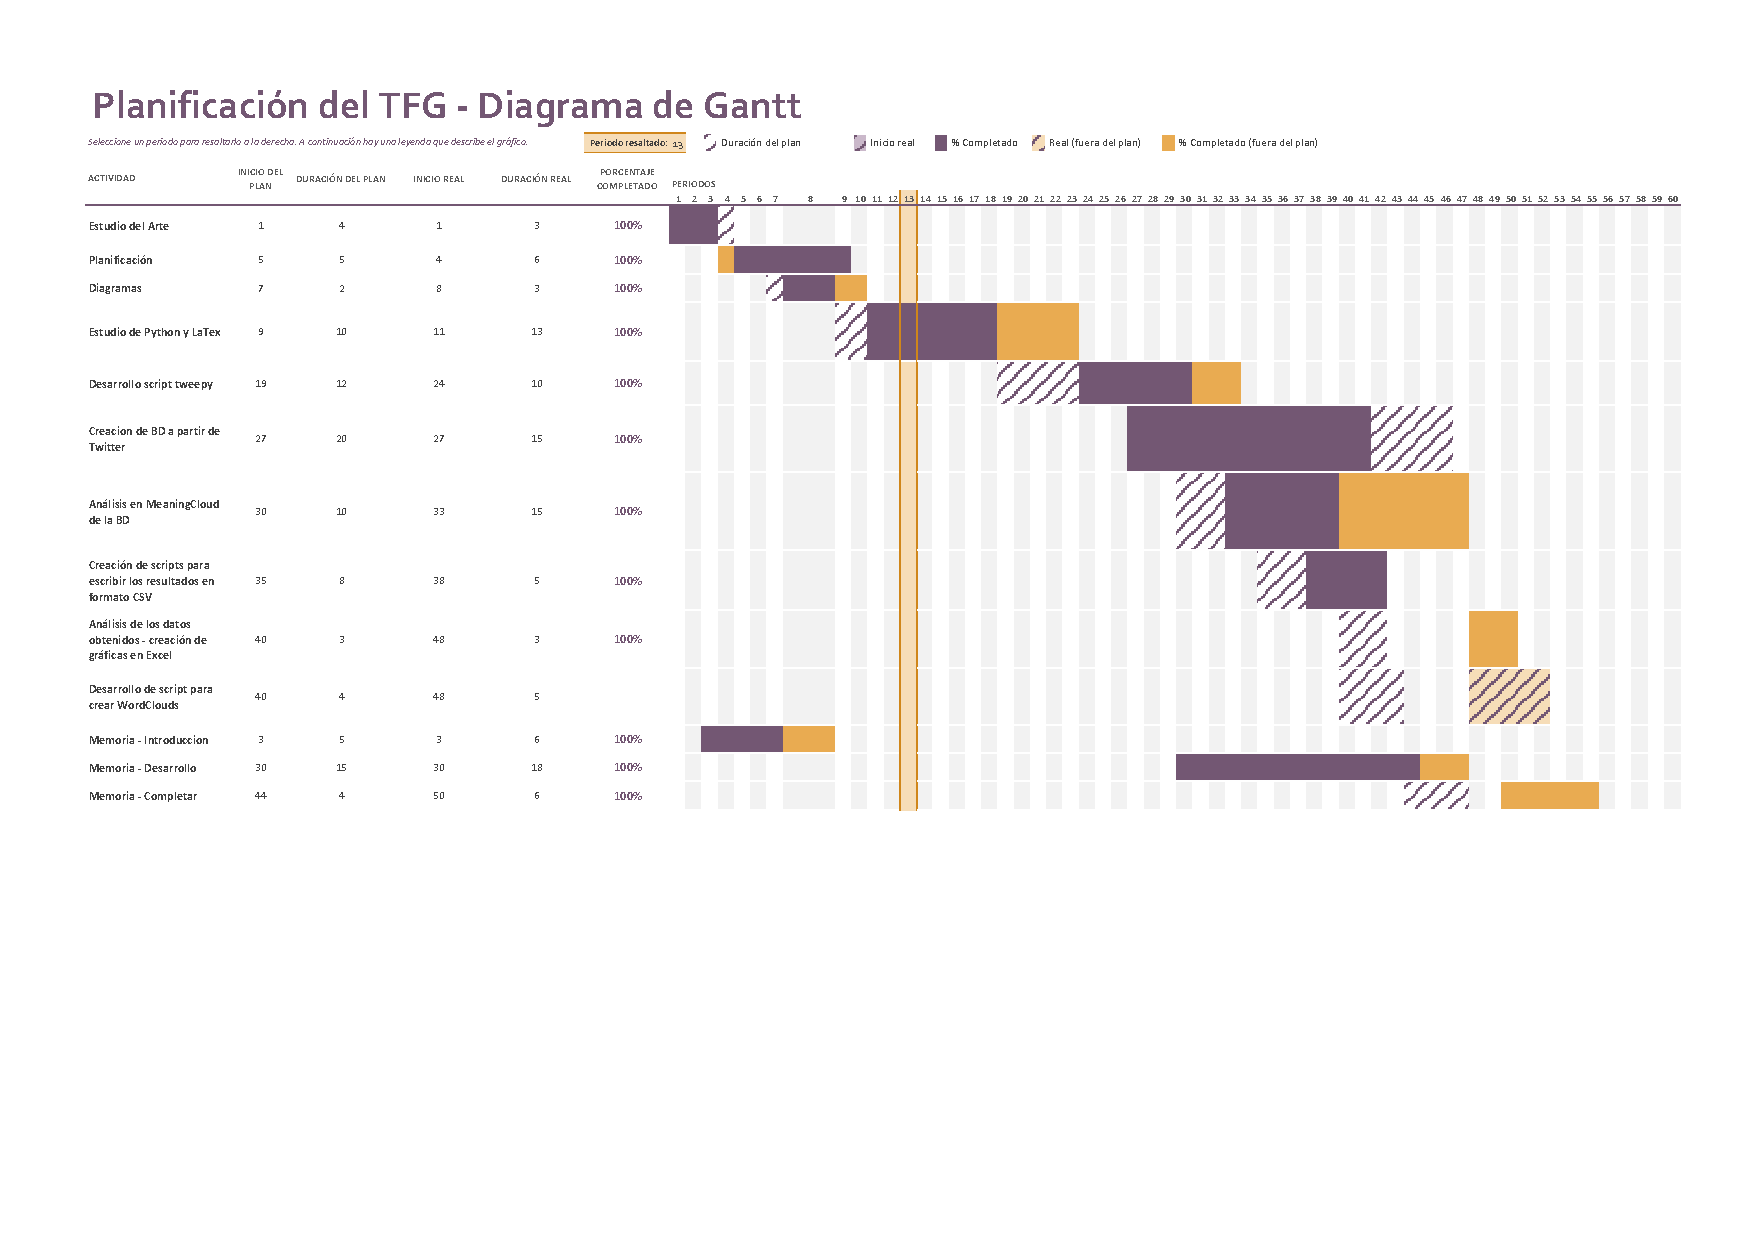
\includepdf[pages={1}]{capitulos/Gantt1-wordcloud.pdf}
En el siguiente diagrama de Gantt aparece la división de trabajo dividido entre la planificación estimada y el tiempo real de realización. Los números que aparecen en la parte superior son las horas de trabajo. Se le estimaron 48 horas en total, teniendo en cuenta que había partes del proceso que podían realizarse simultáneamente. (Mientras se descargan tweets se puede trabajar en otro script que será necesario después). Pero el resultado real, como viene destacado, fue de 56 horas de trabajo. El resto de elementos de la tabla se encuentran en la leyenda del diagrama. 

\begin{figure}[H]
	\centering
	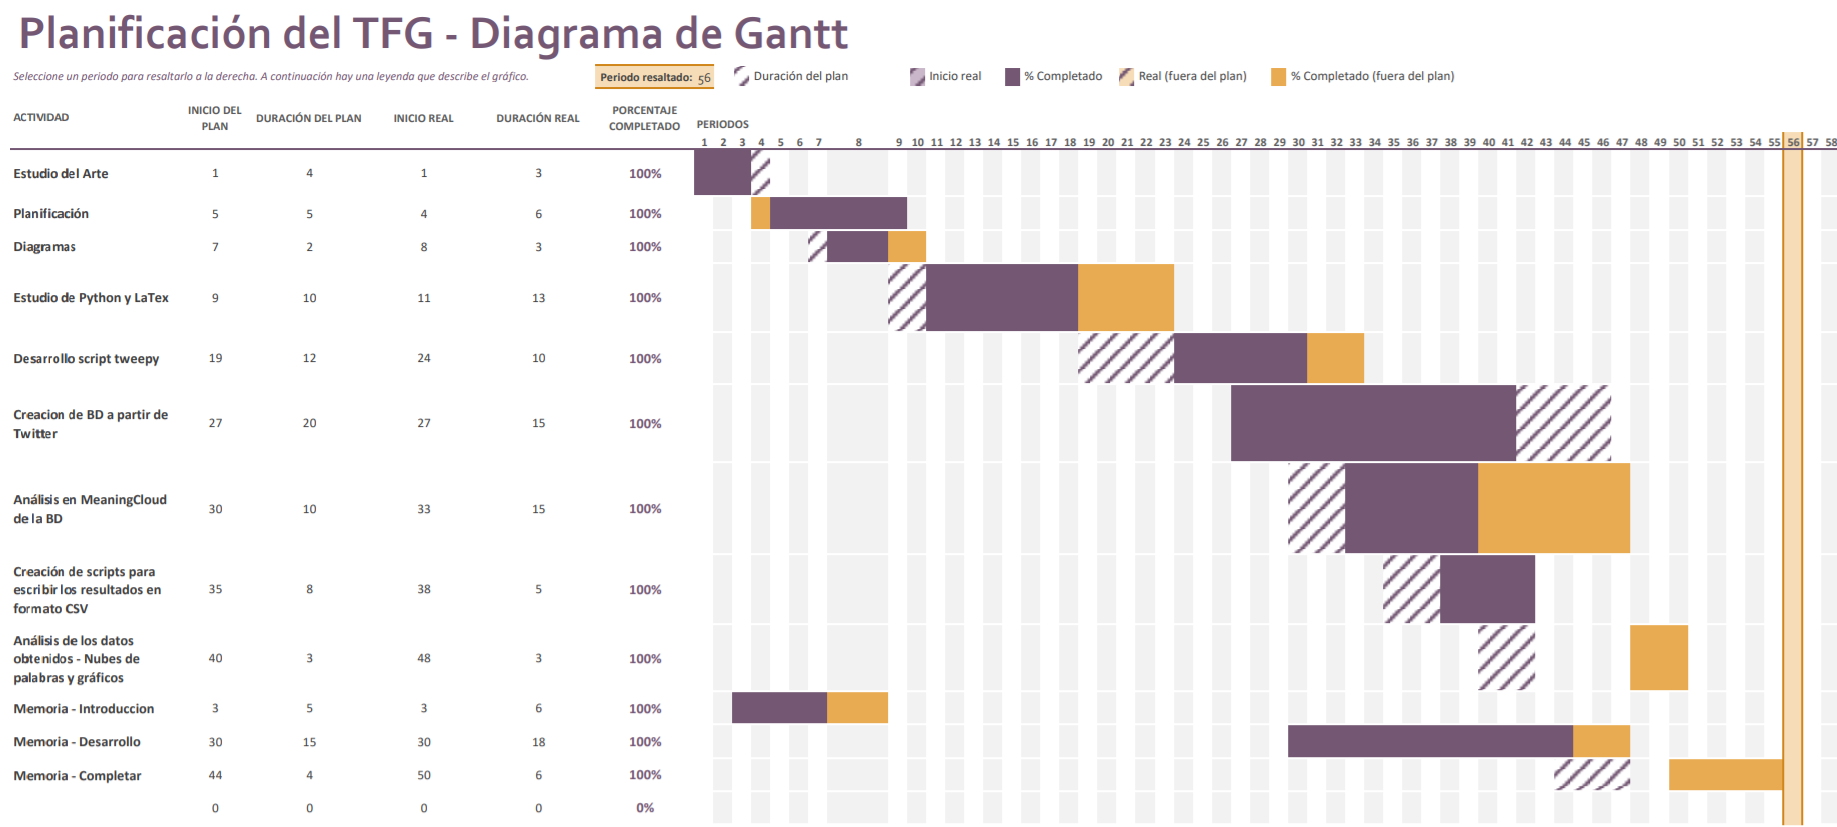
\includegraphics[scale=.45]{imagenes/ganttzoom.png}
	\caption{Diagrama de Gantt}
	\label{fig:gantt}
\end{figure}


















%\input{capitulos/04_Analisis}
%
%%%%%%%%%%%%%%%%%%%%%%%%%%%%%%%%%%%%%%%%%%%%%%%%%%%%%%%%%%%%%%%%%%%%%%%%
% TFG: Vigilancia Tecnológica y Minería de Opiniones en RRSS
% Escuela Técnica Superior de Ingenierías Informática y de Telecomunicación
% Realizado por: Miguel Keane Cañizares
% Contacto: miguekeca@correo.ugr.es 
%%%%%%%%%%%%%%%%%%%%%%%%%%%%%%%%%%%%%%%%%%%%%%%%%%%%%%%%%%%%%%%%%%%%%%%%

\chapter{Presupuesto}


En la planificación del proyecto, se ha estimado una duración de 48 horas para la realización de este proyecto. Basándonos en dicha información, asumiendo un sueldo de Programador Junior de 8 euros la hora, a un cliente se le daría un presupuesto de 384€ por el trabajo a realizar. Las herramientas necesarias son un ordenador personal, el cual ya poseo. Todo el software utilizado es gratuito, aunque si se desean más créditos de MeaningCloud hay que pagar mensualidades, siendo la más barata de 99€ al mes. Los gastos extras son la luz y el wifi necesarios, gastos los cuales son despreciables dentro de mis gastos personales.

Después en la realidad, aunque el trabajo real ha sido de 56 horas, al no haber estimado correctamente los tiempos habría un desajuste de 64€ cobrados de menos. 
%%%%%%%%%%%%%%%%%%%%%%%%%%%%%%%%%%%%%%%%%%%%%%%%%%%%%%%%%%%%%%%%%%%%%%%%
% TFG: Vigilancia Tecnológica y Minería de Opiniones en RRSS
% Escuela Técnica Superior de Ingenierías Informática y de Telecomunicación
% Realizado por: Miguel Keane Cañizares
% Contacto: miguekeca@correo.ugr.es 
%%%%%%%%%%%%%%%%%%%%%%%%%%%%%%%%%%%%%%%%%%%%%%%%%%%%%%%%%%%%%%%%%%%%%%%%

\chapter{Diseño}


El diseño del proyecto tendrá como objetivo mantener la mayor simplicidad y efectividad posible. Para ello primeramente se diseñarán los diferentes requerimientos. 

\subsection{Requerimientos Funcionales}

\begin{itemize}
	\item Registro en la API de Twitter haciendo uso de las credenciales obtenidas.
	\item Introducción de palabras clave para la búsqueda en Twitter.
	\item Seleccionar idioma de los tweets que serán descargados.
	\item Realizar búsquedas de las palabras claves indicadas.
	\item Descargar un tweet y guardarlo en una variable.
	\item Parsear la variable que contenga el tweet en un tipo de dato JSON, más manejable.
	\item Descomposición del Tweet en diferentes variables que contengan la diferente información del mismo.
	\item Aceptar tweets de más de 140 caracteres con el modo \textit{extended\_tweet}.
	\item Creación de base de datos MongoDB con el nombre deseado.
	\item Conexión con la base de datos MongoDB.
	\item Inicialización de colección \textit{tweets} en la base de datos MongoDB.
	\item Almacenamiento de los datos parseados del tweet en un documento MongoDB. 
	
	\item Conexión con la API MeaningCloud con la contraseña proporcionada. 
	\item Introducción del nombre del fichero CSV. 
	\item Comprobación de si el fichero CSV existe con prioridad, de no ser así, crearlo con una primera fila con las caberas de los datos. 
	\item Recorrer la colección \textit{tweets}, enviando uno a uno el cuerpo del tweet a MeaningCloud para ser analizado. 
	\item Almacenamiento y gestión de la respuesta de MeaningCloud.
	\item Distinción entre los diferentes elementos en la respuesta de MeaningCloud. 
	\item Almacenamiento de los datos que se desean conservar del análisis en un fichero CSV y en una nueva colección MongoDB, llamada \textit{concepts}.
	
	\item Creación de nubes de palabras en formato png. 
	\item Creación de gráficas de barras con matplotlib para estudiar los resultados del análisis de sentimientos. 
	\item Introducción de imágenes modelo para la creación de nubes de palabra.
	
	
	
	


\end{itemize}


\subsection{Requerimientos No Funcionales}

\begin{itemize}

	\item Todos las conexiones con Twitter deben tener forma de manejar errores en caso de haberlos. Indicando por pantalla cual ha sido el error y, si es posible, evitar que el programa deje de ejecutarse por el mismo. 
	\item Los datos almacenados deben ser ampliables y reutilizables. 
	\item Evitar los tipos de datos Retweets, ya que estos solo proporcionan información repetida que no será de utilidad para su posterior análisis.
	\item Al almacenar datos en la base de datos, deben preveerse formas de manejar excepciones en caso de error. Priorizando que la ejecución del programa no sea interrumpida y que no haya pérdida de información. 
	
	\item Almacenar las contraseñas en un fichero aparte que será ignorado por Github, para evitar publicar información privada.
	
	\item Manejar posibles errores en la conexión a MeaningCloud, evitando que se interrumpa el proceso de análisis. 
	
	\item Manejar códigos de respuesta de MeaningCloud. Es posible que sin haber un error, el análisis no tenga éxito, se deben manejar estos casos para el programa no interrumpa su ejecución. 
	
	\item Evitar que las comas del texto del tweet sean detectadas como comas separativas en el fichero CSV.
	
	
	
	
	
\end{itemize}



\subsection{Casos de Uso}
Algunos ejemplos de Casos de Uso pueden ser los siguientes: 

\textbf{Conexión a la API de Twitter:}
\begin{itemize}
	\item El usuario solicita conectarse a la API enviando sus credenciales.
	\item El sistema comprueba las credenciales y acepta la conexión. 
	\item El usuario solicita escucha del Stream de tweets que están siendo publicados. 
	\item El sistema devuelve dicho Stream. 
	\item El usuario filtra los resultados para solo descargar los que tengan las palabras clave deseadas en el idioma indicado. 
\end{itemize}


\begin{figure}[H]
	\centering
	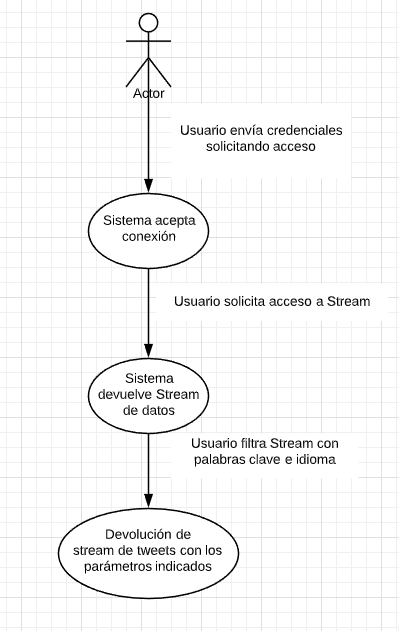
\includegraphics[scale=.4]{imagenes/casoUso1.png}
	\caption{Casos de Uso: Conexión a la API de Twitter.}
	\label{fig:casoUso1}
\end{figure}

\textbf{Conexión a la API de MeaningCloud:}
\begin{itemize}
	\item El usuario solicita conectarse a la API enviando sus credenciales y el texto a analizar
	\item El sistema comprueba las credenciales y analiza el texto. 
	\item El sistema devuelve el resultado del análisis. 
	\item El usuario gestiona los resultados del análisis. 
	\item Si el análisis es exitoso, almacenar los resultados.  
\end{itemize}

\begin{figure}[H]
	\centering
	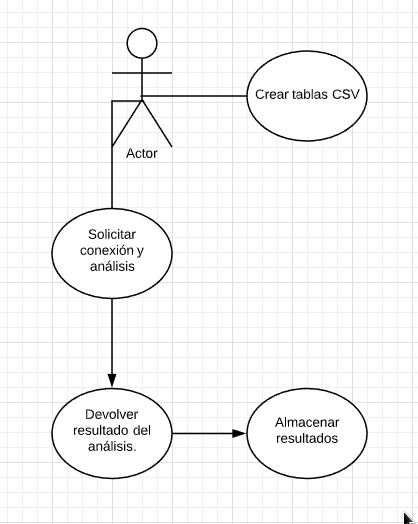
\includegraphics[scale=.4]{imagenes/casoUso2.png}
	\caption{Casos de Uso: Conexión a la API de MeaningCloud.}
	\label{fig:casoUso2}
\end{figure}
%
%%%%%%%%%%%%%%%%%%%%%%%%%%%%%%%%%%%%%%%%%%%%%%%%%%%%%%%%%%%%%%%%%%%%%%%%
% TFG: Vigilancia Tecnológica y Minería de Opiniones en RRSS
% Escuela Técnica Superior de Ingenierías Informática y de Telecomunicación
% Realizado por: Miguel Keane Cañizares
% Contacto: miguekeca@correo.ugr.es 
%%%%%%%%%%%%%%%%%%%%%%%%%%%%%%%%%%%%%%%%%%%%%%%%%%%%%%%%%%%%%%%%%%%%%%%%

\chapter{Implementación}

La mayor parte del proceso de implementación estará enfocado a la creación de los scripts que sean necesarios. Primero implementaremos un programa al que llamaremos \textit{ladrón de tweets} el cual será el encargado de obtener la información de Twitter, crear una base de datos MongoDB y almacernar los datos obtenidos en la misma. 


\subsection{Ladrón de Tweets}

Este código hará uso de las librerías de Tweepy para acceder a la API de Twitter y las librerías de MongoDB para almacenar la información.

\begin{figure}[h]
	\centering
	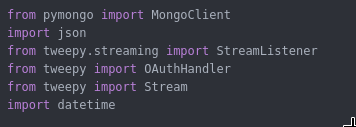
\includegraphics[scale=.6]{imagenes/include-ladron.png}
	\caption{Librerías de ladrón de tweets}
	\label{fig:include-ladron}
\end{figure}


Lo siguiente que hacemos es crear y conectarnos a la base de datos MongoDB, en la cuál almacenaremos toda la información que posteriormente descarguemos. 

\begin{figure}[h]
	\centering
	\includegraphics[scale=1.5]{imagenes/crearMongodb-ladron.png}
	\caption{Inicialización de base de datos MongoDB}
	\label{fig:crear-mongodb}
\end{figure}


Posteriormente es necesario declarar las variables que emplearemos al usar la API de Twitter. El seleccionado, las claves de acceso y las palabras claves que deseamos descargar. 

\begin{figure}[h]
	\centering
	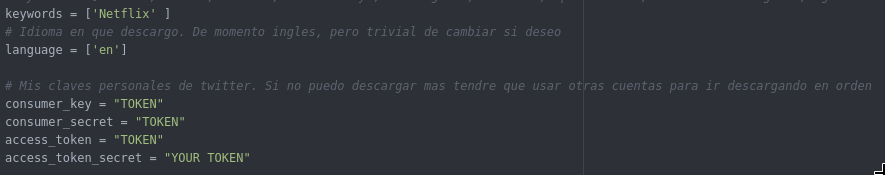
\includegraphics[scale=.4]{imagenes/token-ladron.png}
	\caption{Declaración de variables de acceso, búsqueda e idioma}
	\label{fig:token-ladron}
\end{figure}


Llegado este punto, deberemos hacer la conexión con la API de Twitter mediante las funcionalidades de Tweepy, usando las variables previamente declaradas. Con la función Stream, lo que hacemos es ponerlo en modo escucha, es decir, accederemos a los tweets que sean escritos en el tiempo de ejecución y estos serán los que descarguemos. Debemos incluir el modo \textit{$tweet\_mode$=extended} el cual es necesario porque en caso contrario solo se descargarán los primeros 140 caracteres del tweet, añadiendo información incompleta y por lo tanto desechable en la base de datos. 

\begin{figure}[h]
	\centering
	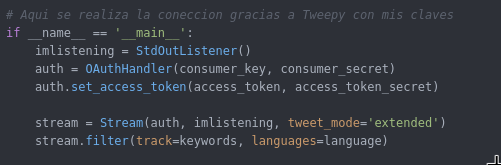
\includegraphics[scale=.5]{imagenes/inicio-sesion-ladron.png}
	\caption{Inicio de sesión en la API de Twitter}
	\label{fig:inicio-sesion-ladron}
\end{figure}


En la función \textit{StdOutListener()} tendremos la parte clave del script, en donde extraeremos la información del tweet y la almacenaremos en MongoDB. Al principio del código evitaremos descargar los Retweets, ya que por experiencia, estos ensucian la base de datos, Esto se debe a que los retweets suponen una repetición, no aportando nueva información, invalidando en parte los resultados de su posterior análisis. 

 
 \begin{figure}[H]
 	\centering
 	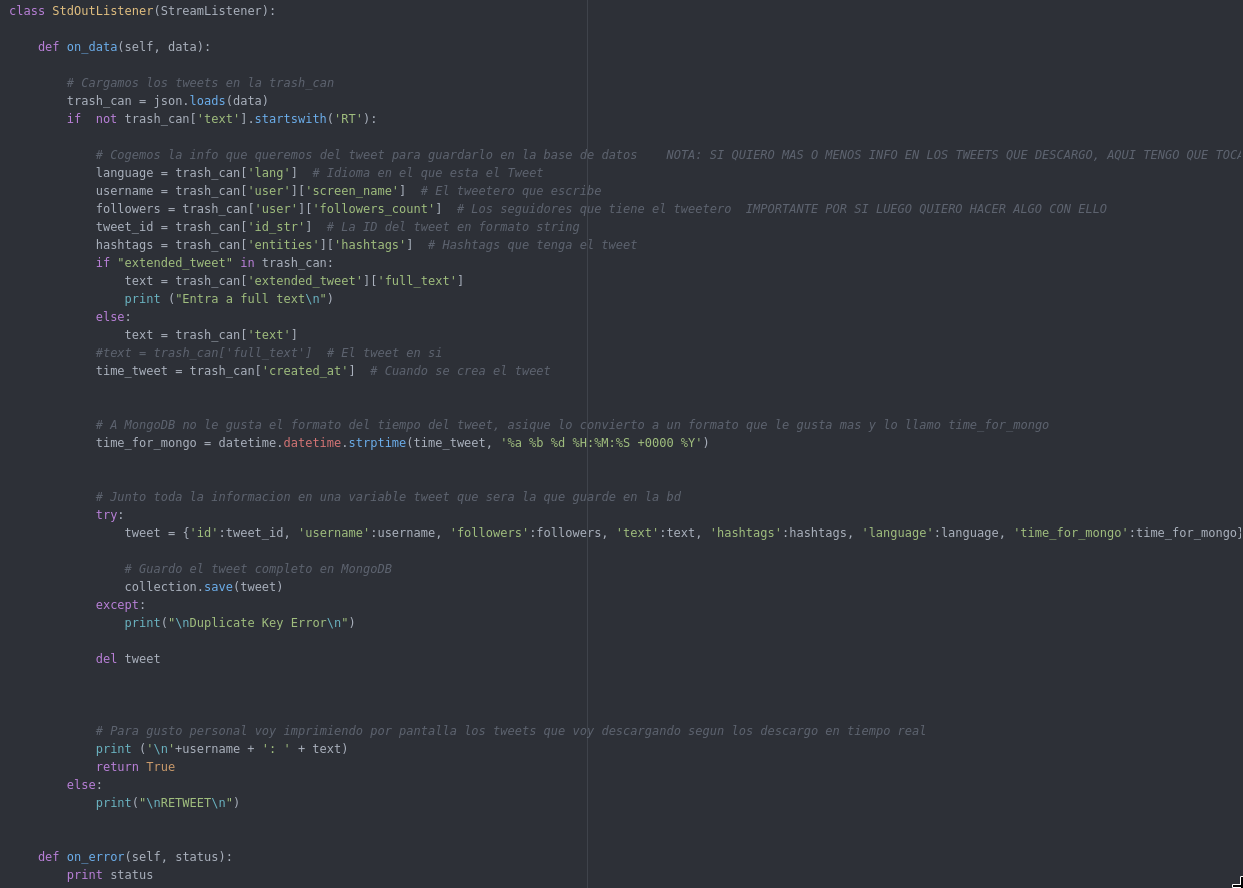
\includegraphics[scale=.35]{imagenes/codigo-ladron.png}
 	\caption{Función de captura y almacenamiento de tweets}
 	\label{fig:codigo-ladron}
 \end{figure}
















\subsection{Análisis de Sentimientos}


Una vez existe una base de datos MongoDB hay que enviarla a analizar a MeaningCloud haciendo uso de su API. Tras su análisis, obtendremos una información que será almacenada por partida doble, para facilitar la reutilización de la misma. Crearemos una colección diferente dentro de la base de datos MongoDB ya existente, a la que denominaremos \textit{concepts} y a la par se creará un archivo CSV en el cual almacenaremos toda la información para facilitar su posterior análisis. 

\begin{figure}[H]
	\centering
	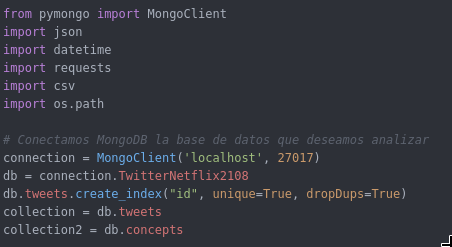
\includegraphics[scale=.35]{imagenes/include-analisis.png}
	\caption{Librerías utilizadas y declaración de la BD y creación de la nueva colección concepts}
	\label{fig:libreria-analisis}
\end{figure}



También será necesario indicar las claves de acceso para la API de MeaningCloud y la dirección url de acceso a la misma. 


\begin{figure}[H]
	\centering
	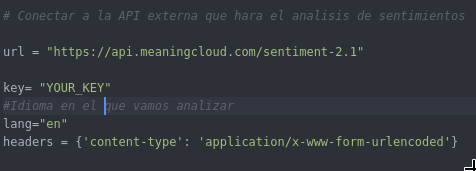
\includegraphics[scale=.35]{imagenes/key-analisis.png}
	\caption{Declaración de variables necesarias para la API de MeaningCloud}
	\label{fig:key-analisis}
\end{figure}




El código recorrerá toda la colección \textit{tweets} de la base de datos MongoDB, mandando únicamente el texto de los tweets a MeaningCloud, pues es la información que deberá ser analizada. Extraemos la información de utilidad de la respuesta y la almacenamos en diferentes variables. Dichas variables son:

\begin{itemize}
	\item \textbf{Confidence:} Es el valor de fiabilidad del análisis. MeaningCloud asigna un valor de 0-100, siendo 100 lo más fiable posible a la calidad de su análisis. Sólo cogeremos los resultados de los análisis aceptables, es decir, que tengan un valor superior a 90.
	\item \textbf{Score\_tag:} Posiblemente la variable más importante del análisis. Puesto que clasificará entre muy positivo y muy negativo el tono emocional del texto analizado. Su rango de polaridad es: 
	\begin{itemize}
		\item P+: Muy positivo
		\item P: Positivo
		\item NEU: Neutral
		\item N: Negativo
		\item N+: Muy negativo
		\item NONE: Ninguno, no se le ha detectado ningún tono emocional al texto.
	\end{itemize}
	\item \textbf{Agreement:} Si hay más de un sentimiento detectado en el texto, si estos sentimientos tienen el mismo tono emocional o no. 
	\item \textbf{Subjectivity:} Subjetividad. Indica si el texto es objetivo o subjetivo.
	\item \textbf{Irony:} Indica si el texto es irónico o no. La experiencia en este proyecto ha aconsejado ignorar esta variable por resultar su tasa de acierto muy baja o nula. 
	\item \textbf{Sentimented\_Entity\_List:} Lista de entidades en el texto que tienen una polaridad, es decir, generan un tono emocional en el autor. Nombres de compañías de servicio, ciudades, países, nombres de usuario. Reconoce un gran rango de entidades. 
	\item \textbf{Sentimented\_Concept\_List:} Lista de conceptos en el texto los cuales tienen polaridad concreta. 
\end{itemize}

Finalmente, tras su análisis. Si la confianza en el mismo está en un rango aceptable, almacenamos los datos en un fichero CSV y en la nueva colección \textit{concepts} que hemos creado dentro de la misma base de datos. Es importante resaltar que este análisis no admite la introducción de emojis, por lo que los tweets que contengan emojis serán devueltos con un mensaje de Error, el cual no interrumpirá el proceso y simplemente seguirá analizando el resto de la base de datos. 


\begin{figure}[H]
	\centering
	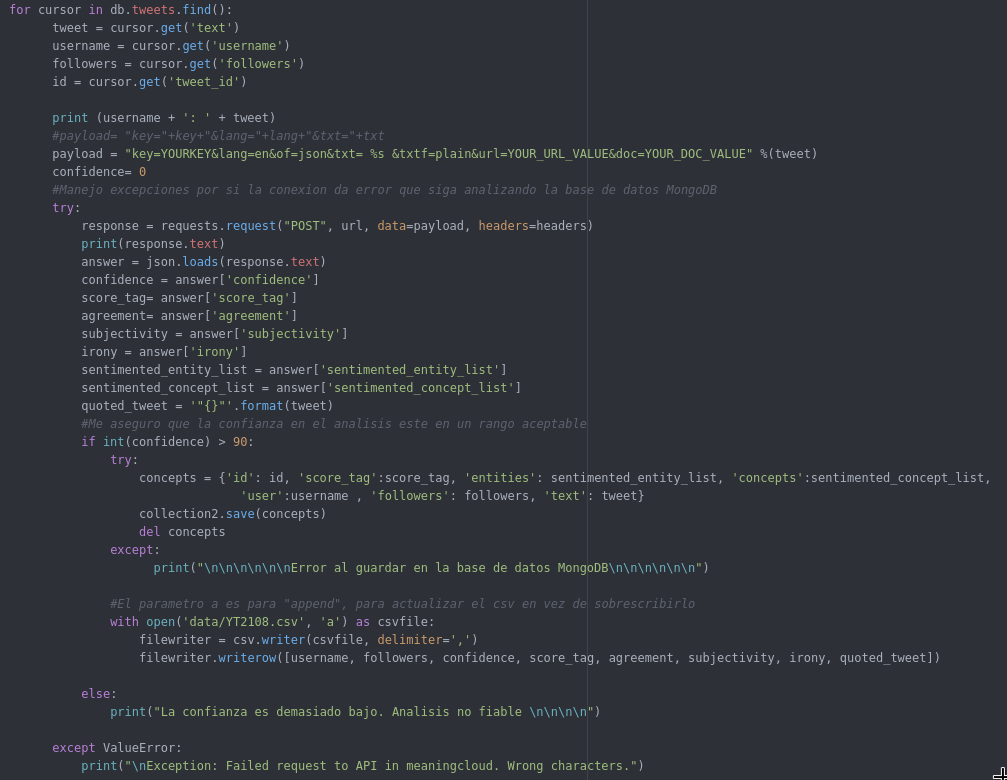
\includegraphics[scale=.35]{imagenes/bucle-analisis.png}
	\caption{Bucle para recorrer la BD de Mongo y analizarla}
	\label{fig:bucle-analisis}
\end{figure}

NOTA: Existe otro script llamado \textbf{analisis-desde-nombre}, el cual es casi idéntico al anteriormente descrito cuya única diferencia es que podemos analizar la base de datos desde un usuario determinado. Por lo que si hay un error, como puede ser una perdida de conexión, será tan trivial como abrir el fichero CSV, buscar el nombre del último usuario añadido al fichero y escribir dicho nombre en la comprobación del script para continuar la búsqueda sin repetir tweets y sin perder información. 



\subsection{WordCloud}

Se ha diseñado un script, que recorrerá todas las palabras de todos los tweets del fichero CSV. Pudiendo con esta información realizar un WordCloud donde aparezcan las palabras más usadas entre todos los tweets. Para ello se hará uso de unas librerías matemáticas de uso científico. Las más importantes serán: 

\begin{itemize}
	\item NumPy: Extensión de python específica para darle mayor soporte para vectores y matrices. Constituye una librería de funciones matemáticas de alto nivel.
	\item Pandas: Estrechamente relacionada con la bibliotea NumPy está orientada a la manipulación y análisis de datos. 	
	\item Matplotlib: biblioteca para la generación de gráficos a partir de datos contenidos en listas o arrays, relacionada también con la extensión NumPy. Diseñada para ser similar a la utilizada en MATLAB
	\item PIL: Python Imaging Lybrary, es una biblioteca que añade soporte para abrir, manipular y almacenar muchos formatos de imagen distintos. 
	
\end{itemize}


\begin{figure}[H]
	\centering
	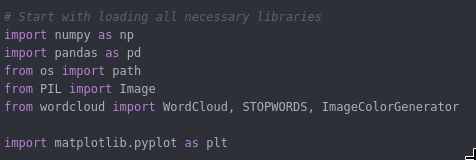
\includegraphics[scale=.5]{imagenes/include-words.png}
	\caption{Librerías utilizadas en el script de WordCloud}
	\label{fig:include-words}
\end{figure}


El código extraerá la información del fichero CSV deseado con la función \textit{read\_csv()} de la librería Pandas. Como información añadida mostrará por pantalla cuantos tweets hay de cada polaridad, desde muy positivo a muy negativo, también hará un recuento de las palabras que haya en la totalidad de los tweets. Los cuales se unificarán todos en una sola variable denominada text gracias a un bucle y a la facilidad de manipulación de datos que ofrece Pandas.
 
 Finalmente para este fragmento, se le introduce una imagen previamente seleccionada, la cual hará de plantilla para la posterior generación del WordCloud, es decir, en vez de usar la forma en la que aparece por defecto, empleará la forma y colores de dicha imagen. La imagen deberá estar en formato RPG, pues gracias a Numpy se generará una máscara con ella transformada en un array de datos. La función array de Numpy convierte la imagen en un vector de datos comprendidos en un rango de 0-255 que contendrán la información de la misma en un formato que el algoritmo pueda procesar.

\begin{figure}[H]
	\centering
	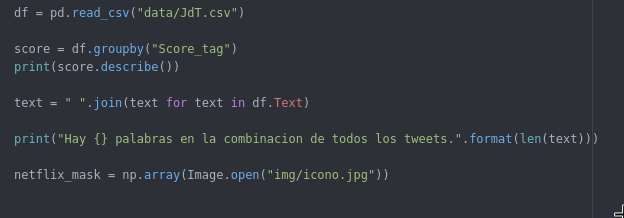
\includegraphics[scale=.5]{imagenes/lectura-imagen-words.png}
	\caption{Lectura de la imagen de plantilla y unificación de todos los tweets en una única variable}
	\label{fig:include-words}
\end{figure}


Una opción para la creación del WordCloud es la asignación de Stopwords, los cuales serán palabras que no se mostrarán en el fichero que se cree. Puesto que hay palabras que debido al formato de los tweets son propensas a aparecer mucho, podemos quitarlas para obtener un WordCloud más satisfactorio. Por ejemplo, si tengo una base de datos acerca de Netflix, es asumible que todos los tweets contendrán la palabra Netflix, sabiendo esto incluimos a Netflix entre los Stopwords para que en el fichero generado veamos las palabras más usadas para hablar de la plataforma, no la plataforma en sí. 

\begin{figure}[H]
	\centering
	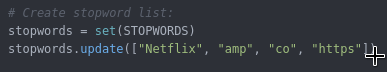
\includegraphics[scale=.7]{imagenes/stopword.png}
	\caption{Adición de Stopwords al WordCloud}
	\label{fig:stopwords}
\end{figure}


Por último, es preciso la generación del WordCloud en sí. Llamando a la función \textit{WordCloud()} en la que introducimos los parámetros deseados, entre los que destacan el número máximo de palabras que generaremos, la máscara que indicará la forma que debe tomar el wordcloud, los stopwords que se han añadido con prioridad, el grosor de los bordes (de tenerlos) de la plantilla y el color de dichos bordes. Con la función \textit{ImageColorGenerator()} a la cual se le añade como parámetro la máscara generada con NumPy, indicará qué colores tomarán las palabras al pintar la figura. Para finalizar, con las funcionalidades de Matplotlib se pintará la imagen, habiendo de indicarle el tamaño de la figura resultante y pasarle la variable de wordcloud que contiene las palabras y por parámetro el color que deseamos que tengan dichas palabras para respetar el formato original. Finalmente, guarda la figura con el nombre y formato deseado y la muestra por pantalla. 

\begin{figure}[H]
	\centering
	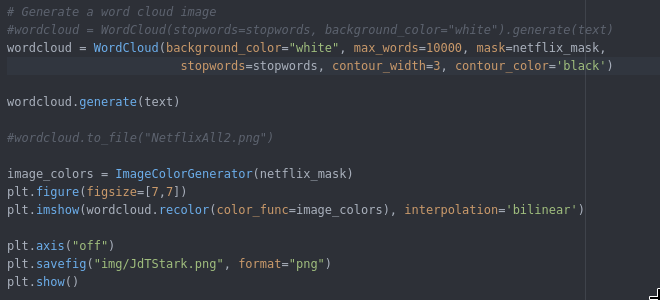
\includegraphics[scale=.5]{imagenes/generar-words.png}
	\caption{Generación de la imagen del WordCloud}
	\label{fig:generacion-words}
\end{figure}













%
%%%%%%%%%%%%%%%%%%%%%%%%%%%%%%%%%%%%%%%%%%%%%%%%%%%%%%%%%%%%%%%%%%%%%%%%
% TFG: Vigilancia Tecnológica y Minería de Opiniones en RRSS
% Escuela Técnica Superior de Ingenierías Informática y de Telecomunicación
% Realizado por: Miguel Keane Cañizares
% Contacto: miguekeca@correo.ugr.es 
%%%%%%%%%%%%%%%%%%%%%%%%%%%%%%%%%%%%%%%%%%%%%%%%%%%%%%%%%%%%%%%%%%%%%%%%

\chapter{Resultados}

De los varios scripts implementados, se han obtenido una gran gama de resultados. Las pruebas han sido orientadas hacia servicios de Streaming Online, debido a que son empresas que están a la orden del día y generan gran actividad en las redes sociales. Con el deseo de buscar una finalidad práctica para realizar un estudio de mercado. Se ha utilizado un formato de \"carreras\" donde se han seleccionado dos plataformas, para las cuales se han ejecutado dos procesos paralelos, cada uno creando una base de datos sobre una plataforma concreta. De esta forma a parte de los resultados de la polaridad, también se puede medir el tráfico de datos que genera su red social con respecto a su competencia. La API de Twitter nos permite hacer dos escuchas simultáneas, por lo que no es necesario hacer uso de más cuentas. 

En total fueron bastantes las bases de datos generadas con las diferentes pruebas, las bases de datos MongoDB generadas fueron las siguientes:


\begin{figure}[H]
	\centering
	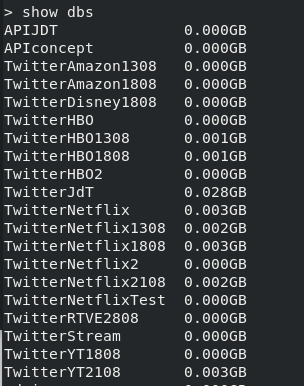
\includegraphics[scale=.5]{imagenes/BD-Mongo.png}
	\caption{Diferentes BD generadas en MongoDB}
	\label{fig:BD-MongoDB}
\end{figure}


\section{Análisis de Netflix y HBO}
Al ser las dos plataformas principales y grandes competidoras entre sí, han sido el objeto principal de las pruebas del proyecto.

La primera competencia fue el día 13 de Agosto, de 22h a 1h. Tres horas donde fueron descargados por separados aquellos tweets que mencionaban Netflix y los que mencionaban a HBO, guardados en diferentes bases de datos. 

\begin{figure}[H]
	\centering
	\begin{tabular}{c c}
		
		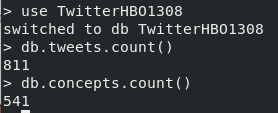
\includegraphics[scale=.62]{imagenes/HBO1308Mongo.png}
		&  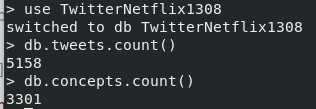
\includegraphics[scale=.65]{imagenes/Netflix1308Mongo.png} \\ 
		
		{BD de HBO1308}
		
		&  {BD de Netflix1308} \\ 
		
	\end{tabular} 
	\label{fig:Mongo1308}
\end{figure}

Aquí podemos apreciar dos colecciones en cada base de datos. La primera \textit{tweets} son el total de tweets capturados por el \textit{ladrón de tweets}, la otra \textit{concepts} son el resultados del análisis de haberlo enviado a MeaningCloud con el \textit{analisis-sentimientos-mongo}. Lo principal que se puede apreciar es que Netflix tiene mucha más presencia en redes que HBO, puesto que es mencionado más de 5 veces por cada vez que se menciona a HBO. 

Tambiés es notable como el número de tweets que han sido analizados es mucho más bajo que los capturados. Esto es debido principalmente a que MeaningCloud no admite emojis en su análisis y siendo estos tan presentes en las redes hay una notable pérdida de información a la hora de analizarla. En este caso los tweets de HBO han tenido una tasa del 66,7\% de tweets analizables mientras que Netflix tiene una tasa del 64\%. La diferencia es casi despreciable. 


Pasando a estudiar los resultados del análisis de sentimientos, obtenemos lo siguiente. 

\begin{table}[H]
	\centering
	\begin{tabular}{|c|c|c|}
		\hline 
		Polaridad& Suma de polaridades & Porcentaje \\ 
		\hline 
		N+& 36 & 10,62\% \\ 
		\hline 
		N& 90 &  26,55\%\\ 
		\hline 
		NEU& 17 & 5,01\% \\ 
		\hline 
		P& 154 & 45,43\% \\ 
		\hline 
		P+& 42 & 12,39\% \\ 
		\hline 
		Total & 339 & \\
		\hline
	\end{tabular} 
	\caption{Tabla de porcentajes de HBO1308}
	\label{tbl:porcentaje-HBO1308}
\end{table}



La razón por la que en el total de aparece la cifra de 339 en vez de 541 es porque 202 tweets han sido clasificados como NONE, es decir, sin ninguna polaridad emocional detectada. Esto correspondería al 37\% de los tweets analizados.

\begin{table}[H]
	\centering
	\begin{tabular}{|c|c|c|}
		\hline 
		Polaridad& Suma de polaridades & Porcentaje \\ 
		\hline 
		N+& 292 & 14,37\% \\ 
		\hline 
		N& 920 &  42,28\%\\ 
		\hline 
		NEU& 134 & 6,59\% \\ 
		\hline 
		P& 527 & 25,94\% \\ 
		\hline 
		P+& 159 & 7,82\% \\ 
		\hline 
		Total & 2032 & \\
		\hline
		
	\end{tabular} 
	\caption{Tabla de porcentajes de Netflix1308}
	\label{tbl:porcentaje-Netflix1308}
\end{table}
\begin{figure}[H]
	
\end{figure}



En Netflix el 38\% de los tweets analizados no tenían polaridad. Equivalente a 1269 tweets de los 3301 estudiados. 

A continuación ilustraremos unos gráficos de los resultados: 

\begin{figure}[H]
	\centering
	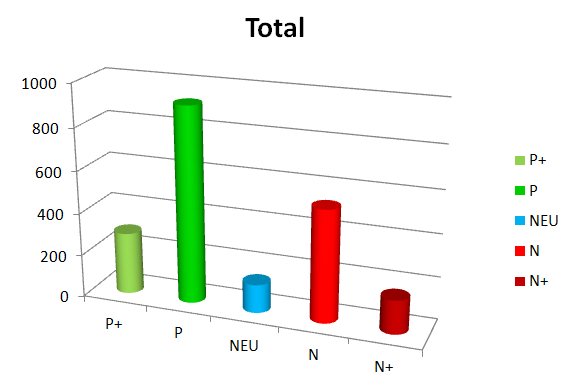
\includegraphics[scale=.3]{imagenes/GraficoBarrasNetflix1308.PNG}
	\caption{Gráfico de barras de Netflix1308}
	\label{fig:barrasNetflix1308}
\end{figure}


\begin{figure}[H]
	\centering
	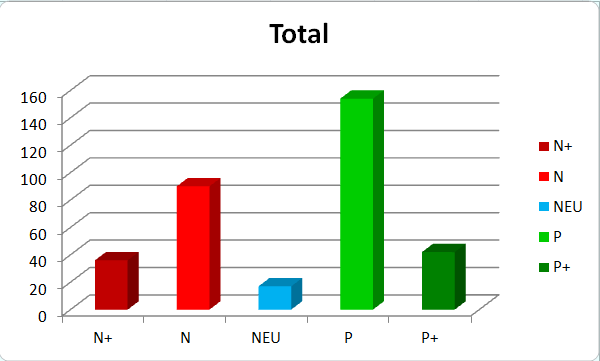
\includegraphics[scale=.3]{imagenes/barrasHBO1308.PNG}
	\caption{Gráfico de barras de HBO1308}
	\label{fig:barrasHBO1308}
\end{figure}

Con estos resultados podemos apreciar que la mayoría de los tonos emocionales detectados son Negativos o Positivos, siendo los positivos la mayoría tanto en Netflix como en HBO. 


El siguiente análisis fue realizado el 18 de Agosto de 2019. desde las 0:20 hasta las 3am. Un total de dos horas y cuarenta minutos. 

\begin{figure}[H]
	\centering
	\begin{tabular}{c c}
		
		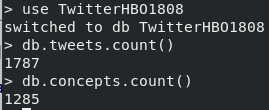
\includegraphics[scale=.7]{imagenes/HBO1808Mongo.png}
		&  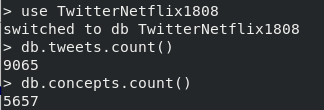
\includegraphics[scale=.7]{imagenes/Netflix1808Mongo.png} \\ 
		
		{BD de HBO1808}
		
		&  {BD de Netflix1808} \\ 
		
	\end{tabular} 
	\label{fig:Mongo1808}
\end{figure}

Netflix no deja lugar a dudas, vuelve a tener 5 veces más tráfico en las redes que su rival HBO. 
En esta ocasión, HBO ha tenido un 72\% de tweets sin emojis y Netflix se mantiene casi igual que antes con un 62\%. Analizando los resultados uno por uno se observa lo siguiente: 

\begin{table}[H]
	\centering
	\begin{tabular}{|c|c|c|}
		\hline 
		Polaridad& Suma de polaridades & Porcentaje \\ 
		\hline 
		N+& 265 & 7.87\% \\ 
		\hline 
		N& 815 &  24.21\%\\ 
		\hline 
		NEU& 237 & 7.04\% \\ 
		\hline 
		P& 1435 & 42.63\% \\ 
		\hline 
		P+& 614 & 18.24\% \\ 
		\hline 
		Total & 3366 & \\
		\hline
	\end{tabular} 
	\caption{Tabla de porcentajes de Netflix1808}
	\label{tbl:porcentaje-Netflix1808}
\end{table}

En Netflix a 2291 tweets, es decir, al 60\% de los analizados, no se le ha detectado tono emocional alguno. 

\begin{table}[H]
	\centering
	\begin{tabular}{|c|c|c|}
		\hline 
		Polaridad& Suma de polaridades & Porcentaje \\ 
		\hline 
		N+& 73 & 9.22\% \\ 
		\hline 
		N& 220 &  27.78\%\\ 
		\hline 
		NEU& 67 & 8.46\% \\ 
		\hline 
		P& 357 &45.08\% \\ 
		\hline 
		P+& 75 & 9.47\% \\ 
		\hline 
		Total & 792 & \\
		\hline
	\end{tabular} 
	\caption{Tabla de porcentajes de HBO1808}
	\label{tbl:porcentaje-HBO1808}
\end{table}
HBO ha tenido 493 tweets sin tono emocional, equivalente aproximadamente al 38\% del total analizado. 


Las gráficas obtenidas son las siguientes: 

\begin{figure}[H]
	\centering
	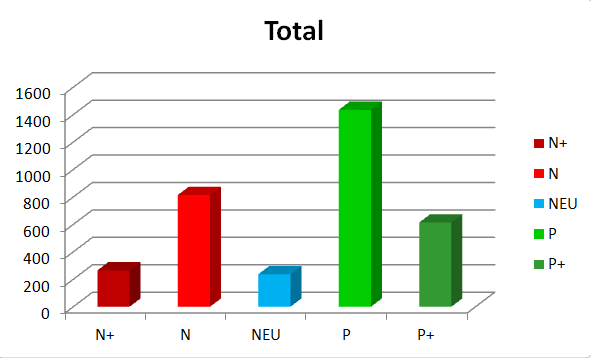
\includegraphics[scale=.3]{imagenes/barrasNetflix1808.PNG}
	\caption{Gráfico de barras de Netflix1808}
	\label{fig:barrasNetflix1808}
\end{figure}



\begin{figure}[H]
	\centering
	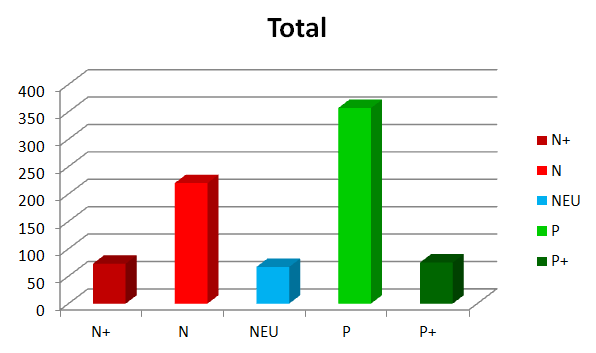
\includegraphics[scale=.3]{imagenes/barrasHBO1808.PNG}
	\caption{Gráfico de barras de HBO1808}
	\label{fig:barrasHBO1808}
\end{figure}


Aquí se observa la misma tendencia anterior, la inmensa mayoría de la polaridad emocional es para expresar un tono positivo o negativo, pocos expresan polaridades extremas o neutras. Con la diferencia de que en HBO hay un incremento del porcentaje de opiniones negativas con respecto a Netflix y Netflix porcentualmente recibe cerca del doble de tonos muy positivos. 


\subsection{Netflix vs Youtube}

Al haber observado que Netflix poseía una abrumadora superioridad en cuanto a número de usuarios y actividad en las redes que HBO, se optó por hacerla competir con una plataforma mucho más grande, como puede ser YouTube. YouTube es otro formato de plataforma de Streaming Online, pero a diferencia de Netflix y HBO su contenido es gratuito y creado por los propios usuarios, aunque recientemente se ha presentado al público YouTube Premium, cuya ventaja es la de suprimir los anuncios, han aprovechado para empezar a ofrecer contenido cinematográfico exclusivo para sus suscriptores, es decir, series y películas producidas por la compañía de Google, como llevan muchos años haciendo Netflix y HBO. 

Se les analizó el 21 de Agosto de 2019, de las 16h hasta las 17:30h. Una hora y media de escucha.


 
 \begin{figure}[H]
 	\centering
 	\begin{tabular}{c c}
 		
 		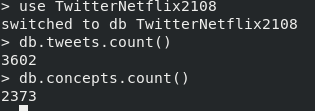
\includegraphics[scale=.7]{imagenes/Netflix2108Mongo.png}
 		&  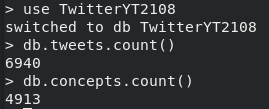
\includegraphics[scale=.7]{imagenes/YT2108Mongo.png} \\ 
 		
 		{BD de Netflix2108}
 		
 		&  {BD de YouTube2108} \\ 
 		
 	\end{tabular} 
 	\label{fig:Mongo2108}
 \end{figure}


Es apreciable, que siempre hay un pez más grande. YouTube en tan solo hora y media es mencionada el doble de veces que Netflix.  Netflix mantiene su línea de contenido sin emojis, un 65,8\% de todos los tweets son analizables, mientras que YouTube se mantiene superior, con un 70\% de éxito en los tweets que se analizan correctamente. 



\begin{table}[H]
	\centering
	\begin{tabular}{|c|c|c|}
		\hline 
		Polaridad& Suma de polaridades & Porcentaje \\ 
		\hline 
		N+& 96 & 6.71\% \\ 
		\hline 
		N& 358 &  25.02\%\\ 
		\hline 
		NEU& 102 & 7.13\% \\ 
		\hline 
		P& 646 & 45,14\% \\ 
		\hline 
		P+& 229 & 16.00\% \\ 
		\hline 
		Total & 1431 & \\
		\hline
	\end{tabular} 
	\caption{Tabla de porcentajes de Netflix2108}
	\label{tbl:porcentaje-Netflix2108}
\end{table}

En Netflix ha habido 942 tweets sin tono emocional, lo que equivale al 39,69\% de los analizados. 

\begin{table}[H]
	\centering
	\begin{tabular}{|c|c|c|}
		\hline 
		Polaridad& Suma de polaridades & Porcentaje \\ 
		\hline 
		N+& 238 & 8.38\% \\ 
		\hline 
		N& 773 &  27.22\%\\ 
		\hline 
		NEU& 135 & 4.75\% \\ 
		\hline 
		P& 1327 & 46.73\% \\ 
		\hline 
		P+& 367 & 12.92\% \\ 
		\hline 
		Total & 2840 & \\
		\hline
	\end{tabular} 
	\caption{Tabla de porcentajes de YouTube2108}
	\label{tbl:porcentaje-YT2108}
\end{table}

En YouTube hubo 2073 tweets carentes de tono emocional, 42,12\% del total. 


\begin{figure}[H]
	\centering
	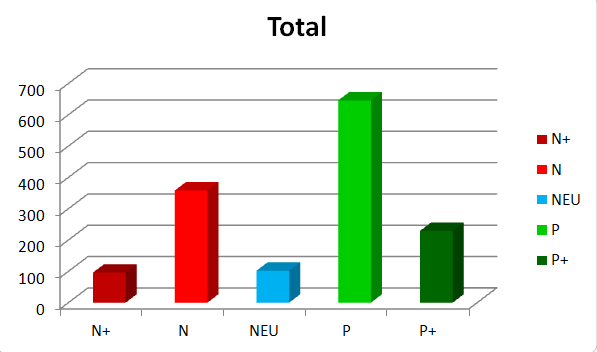
\includegraphics[scale=.3]{imagenes/barrasNetflix2108.PNG}
	\caption{Gráfico de barras de Netflix2108}
	\label{fig:barrasNetflix2108}
\end{figure}



\begin{figure}[H]
	\centering
	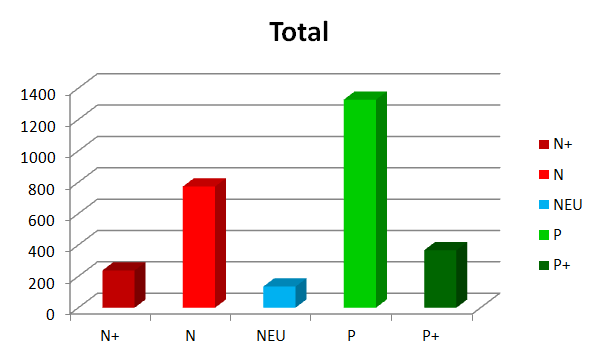
\includegraphics[scale=.3]{imagenes/barrasYT2108.PNG}
	\caption{Gráfico de barras de YouTube2108}
	\label{fig:barrasYT2108}
\end{figure}


En cuanto a las gráficas se refieren, no hay diferencias notables entre las dos plataformas. Se mantiene el tono positivo a la cabeza con el negativo detrás. Aunque levemente, en YouTube hay un mayor porcentaje de tonos extremos, es decir, hay más tonos muy positivos y tonos muy negativos que en Netflix. 



\subsection{Estudio del total analizado}
Uniendo todos los tweets analizados en ficheros únicos gracias al script \textit{unificador-csv} para poder analizar los resultados completos.


\textbf{Netflix: }

\begin{table}[H]
	\centering
	\begin{tabular}{|c|c|c|}
		\hline 
		Polaridad& Suma de polaridades & Porcentaje \\ 
		\hline 
		N+& 520 & 7.61\% \\ 
		\hline 
		N& 1700 &  24.89\%\\ 
		\hline 
		NEU& 473 & 6.93\% \\ 
		\hline 
		P& 3001 & 43.94\% \\ 
		\hline 
		P+& 1135 & 16.62\% \\ 
		\hline 
		Total & 6829 & \\
		\hline
	\end{tabular} 
	\caption{Tabla de porcentajes de Netflix total}
	\label{tbl:porcentaje-NetflixAll}
\end{table}

 \begin{figure}[H]
	\centering
	
	 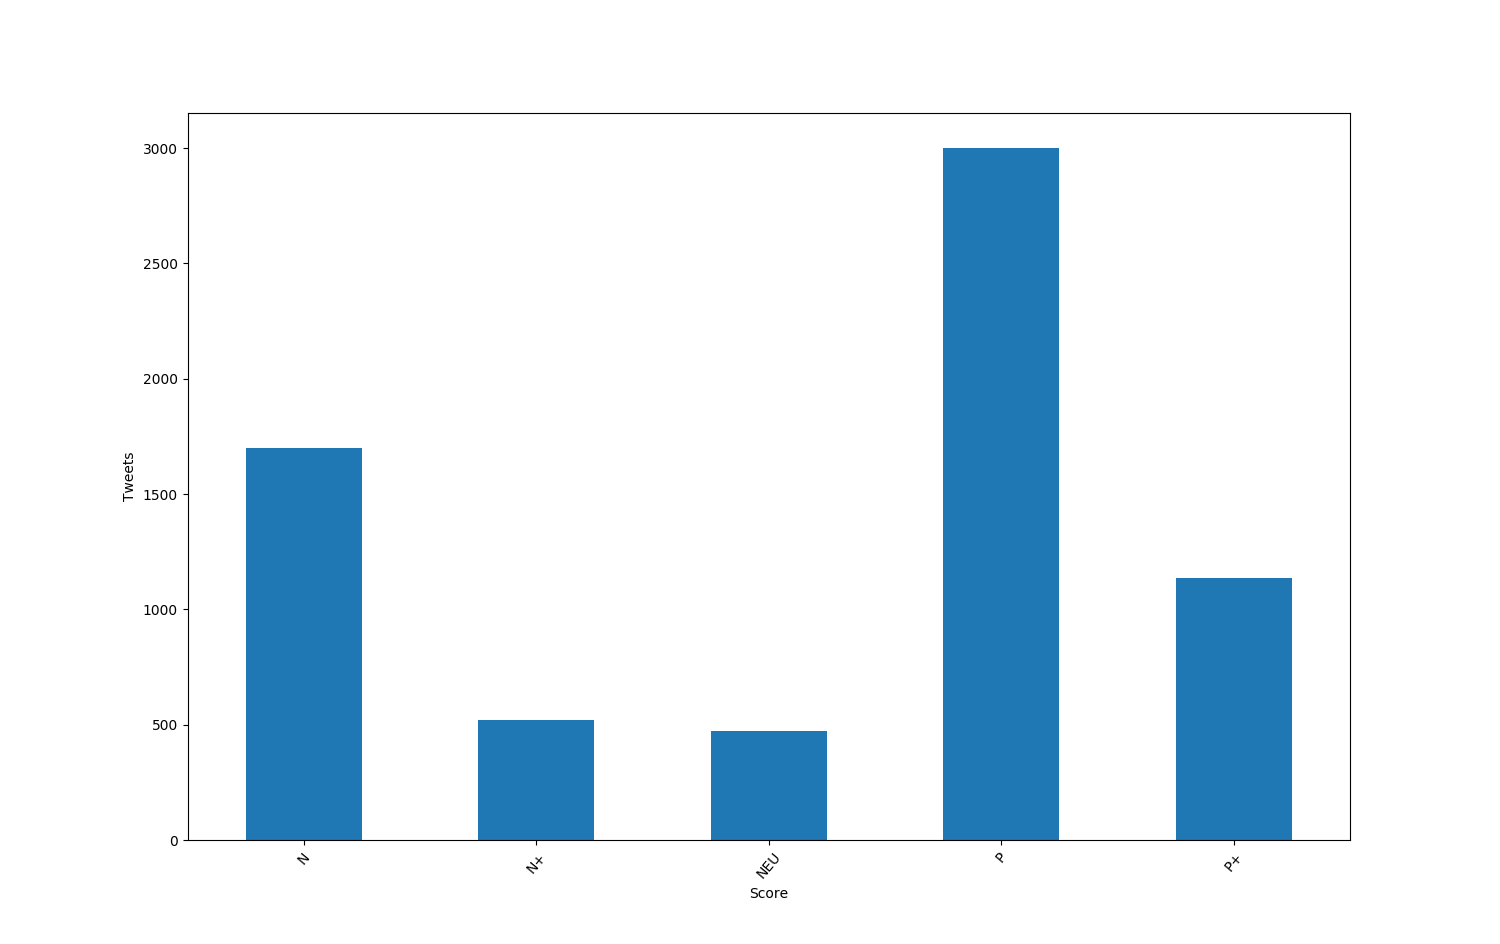
\includegraphics[scale=.3]{imagenes/barrasNetflixAll.png}
		
	
		
	\caption{Gráfico de barras de Netflix total} 
	\label{fig:NetflixAll}
\end{figure}





Es claramente apreciable que la gran mayoría de los comentarios de Netflix son positivos y muy positivos. Hay más comentarios negativos que muy positivos,  pero la diferencia es mínima y siendo solo el 39\% del total positivo es superior al 19\% que suman los tweets negativos y muy negativos. 




\textbf{HBO: }


\begin{table}[H]
	\centering
	\begin{tabular}{|c|c|c|}
		\hline 
		Polaridad& Suma de polaridades & Porcentaje \\ 
		\hline 
		N+& 116 & 26.76\% \\ 
		\hline 
		N& 320 &  9.70\%\\ 
		\hline 
		NEU& 90 & 7.53\% \\ 
		\hline 
		P& 547 & 45.74\% \\ 
		\hline 
		P+& 123 & 10.28\% \\ 
		\hline 
		Total & 1196 & \\
		\hline
	\end{tabular} 
	\caption{Tabla de porcentajes de HBO total}
	\label{tbl:porcentaje-HBOAll}
\end{table}

\begin{figure}[H]
	\centering
		
		 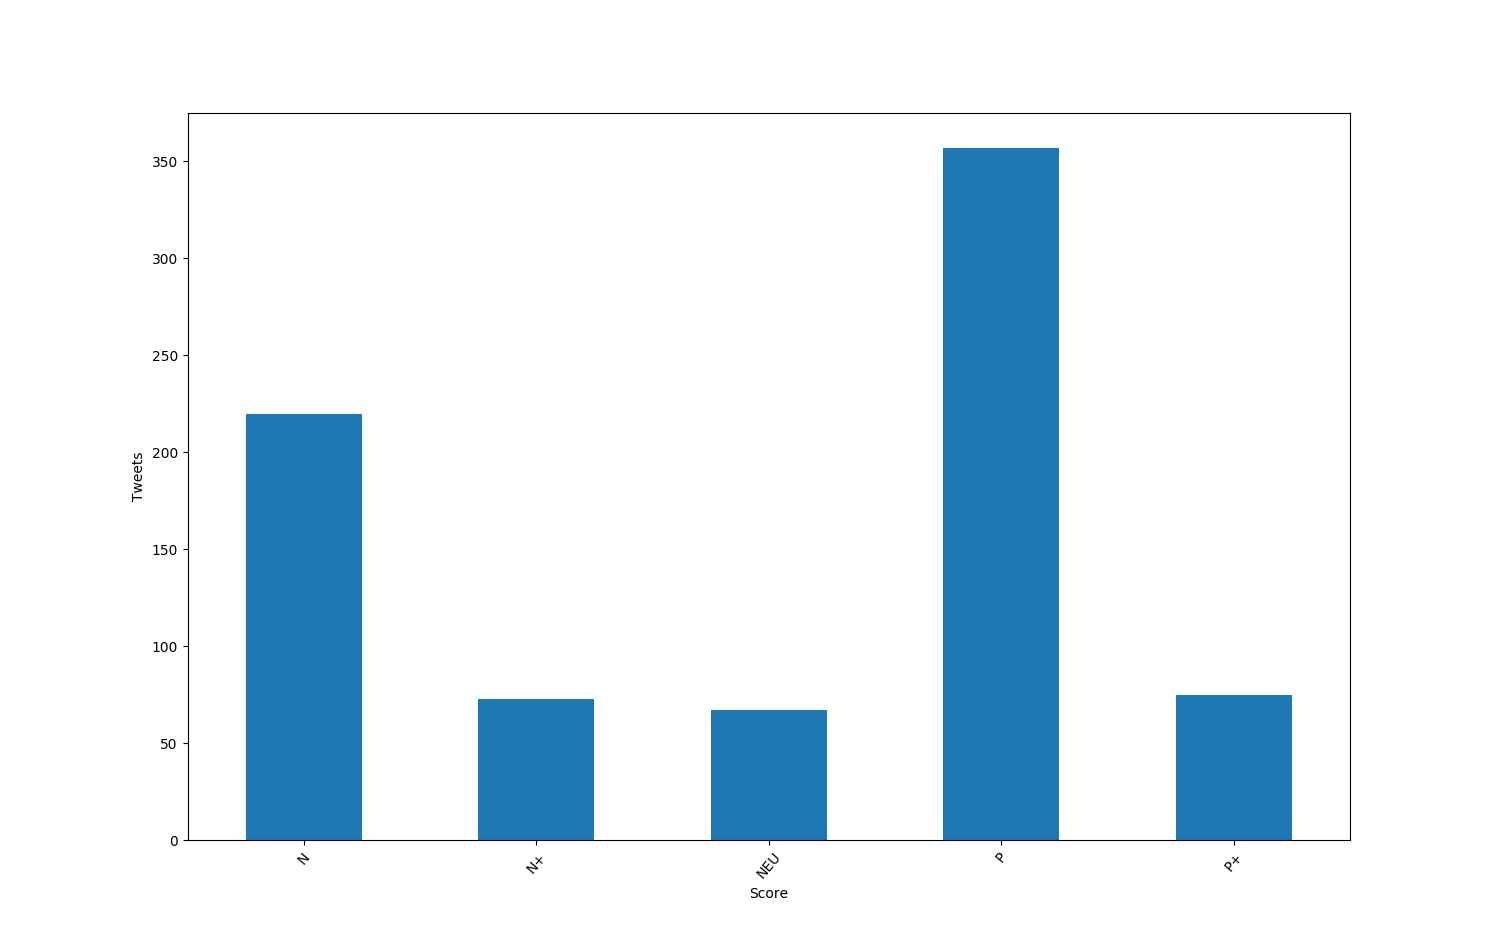
\includegraphics[scale=.3]{imagenes/barrasHBOAll.png} 
		
		{Porcentajes de HBO total}
		
	\caption{Gráfico de barras de HBO total} 
		
	\label{fig:HBOAll}
\end{figure}



La tendencia es similar a la de Netflix, puesto que la mayoría de comentarios son positivos y se evitan los extremos y los neutros. Pero en HBO la diferencia entre positivos y negativos es menor, es decir, hay una mayor porcentaje de usuarios que escriben comentarios negativos al hablar de HBO. 



\subsection{Disney+ y AmazonVideos}

También, como dato anecdótico, se intentó hacer competir la repercusión en redes de la plataforma que va a sacar Disney al mercado, Disney+, y la plataforma de Amazon, AmazonVideos. Pero los resultados fueron poco alentadores, con apenas 150 tweets de Disney+ publicados durante la captación y tan solo 3 tweets de AmazonVideos en el mismo espacio, cabe notar que los tweets de Amazon fueron todos publicados por un mismo usuario repitiendo un mismo mensaje. 



\subsection{WordClouds}
Las nubes de palabras son una forma útil para analizar los datos obtenidos. Con esta forma podemos crear un resumen visual de los datos obtenidos, obteniendo las palabras más utilizadas en la base de datos almacenada. 


Inicialmente las nubes de palabras se veían así: 

\begin{figure}[H]
	\centering
	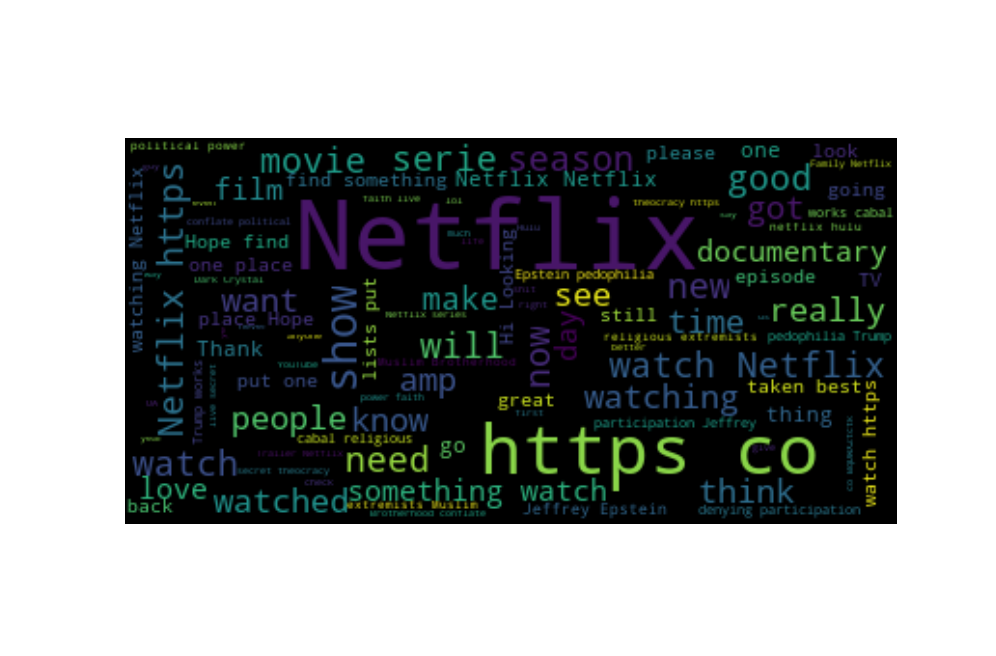
\includegraphics[scale=.5]{imagenes/WordCloudNetflix1.png}
	\caption{Primer WordCloud de Netflix}
	\label{fig:wordcloudNetflix1}
\end{figure} 

El primer fallo notable era que la palabra \textit{Netflix} aparecía muy repetida, lo cual es obvio, pues esta era la palabra clave utilizada para descargar los tweets, es decir, todos ellos la contenían. Además, un gran número de tweets incluye enlaces, al empezar todos los enlaces por https el algoritmo detectó esta palabra apareciendo repetidas veces. Además se detectó \textit{amp}, utilizado por caracteres especiales y \textit{co} que figura en los enlaces. Implementando el uso de stopwords y cambiando el fondo a blanco por limpieza visual el resultado fue el siguiente: 

\begin{figure}[H]
	\centering
	
\includegraphics[scale=.3]{imagenes/NetflixAll.png}
	\caption{Segundo WordCloud de Netflix}
	\label{fig:wordcloudNetflix2}
\end{figure} 

En esta segunda versión, se aumenta el número de palabras representadas y el uso de StopWords para limpiar los resultados. Los resultados obtenidos son los que nos podíamos esperar del análisis de un wordcloud de Netflix, palabras como watch, movie, season entre otras están presentes. Es notable como leyendo los resultados se puede extrapolar como la mayoría de usuarios lo utiliza para hablar de series y programas que le gustan: love, good, watch, now. Y como también hay otros usuarios que comentan para recibir recomendaciones: something watch ,  please, Looking. 

Lo mismo sucedía con los demás, por lo que adaptando las palabras claves este era el resultado: 

\begin{figure}[H]
	\centering
	\includegraphics[scale=.8]{imagenes/ytwords.png}
	\caption{Primer WordCloud de YouTube}
	\label{fig:wordcloudYT1}
\end{figure} 

Y excluyendo la palabra YouTube: 

\begin{figure}[H]
	\centering
	\includegraphics[scale=.8]{imagenes/ytstopwords.png}
	\caption{Segundo WordCloud de YouTube}
	\label{fig:wordcloudYT2}
\end{figure} 


Aquí es apreciable una diferencia del formato. Ya no se ven palabras como season, movie o serie. Las cuales se ven reemplazadas por video, song, subscribe o play. Google, dueña de YouTube aparece mencionada en muchas ocasiones. 
 
Para el estudio de la nube de HBO, además de cambiar los colores se cambiaron los contornos, para mostrar las posibilidades estéticas que permite el manejo de la librería \textbf{PIL}\cite{Pillow}. Siendo posible la creación de nubes con diferentes formas. 

\begin{figure}[h]
	\centering
	
\includegraphics[scale=.75]{imagenes/hbo_color2.png}
	\caption{WordCloud de HBO}
	\label{fig:wordcloudHBO}
\end{figure} 

En cuanto a las palabras, no se aprecia gran diferencia con respecto a las de Netflix, al ser un servicio parecido, inevitablemente aparecen palabras similares. Con el detalle de que aparece mencionada la plataforma Hulu, la cual tras una breve búsqueda en Google podemos averiguar que en Estados Unidos esta plataforma ofrece los servicios de HBO de la misma forma que Movistar ofrece Netflix en España. 




\subsection{Juego de Tronos}

Como añadido, durante la semana del final del último capítulo de la serie Juego de Tronos hubo una versión previa del \textit{ladrón de tweets}, capturó más de 170mil tweets solo en dos días, el problema es que no esta versión no disponía de un filtro para evitar los Retweets, por lo que la inmensa mayoría de la información es el mismo tweet repetido una y otra vez. Además no estaba gestionado el modo extendido para capturar tweets de más de 140 caracteres. Por lo que su utilidad real para el análisis de sentimientos es escasa, pero aún así se ha realizado un wordcloud y un análisis de sentimientos parcial, pues el número de tweets era abrumador. 



El total de palabras analizadas es de 19.809.698, las cuales generan el siguiente wordcloud:

\begin{figure}[H]
	\centering
	
\includegraphics[scale=.7]{imagenes/JdTLogo.png}
	\caption{Wordcloud de Juego de Tronos}
	\label{fig:wordcloudJdT}
\end{figure} 


Cuya versión simplificada, más fácil de leer sería: 
\begin{figure}[H]
	\centering
	\includegraphics[scale=.9]{imagenes/JdTred.png}
	\caption{Wordcloud de Juego de Tronos simple}
	\label{fig:wordcloudJdT}
\end{figure} 

Una de las cosas que más llama la atención de este wordcloud fue la gran presencia de \"Avatar the Last Airbender\" y de \"Snoop Dogg\". Esto se debe a dos tweets diferentes publicados mientras se realizaba la captura de tweets, los cuales obtuvieron una enorme cantidad de Retweets y se almacenaron en la base de datos MongoDB miles de veces. 


\begin{figure}[H]
	\centering
	\begin{tabular}{c c}
		
		
\includegraphics[scale=.3]{imagenes/airbender.png}
		&  
\includegraphics[scale=.3]{imagenes/snoop.png} \\ 
		
		{Tweet de Avatar Last Airbender}
		
		&  {Tweet sobre la reacción de Snoop Dogg} \\ 
		
	\end{tabular} 
	\caption{Tweets que tuvieron una alta tasa de Retweets y ensuciaron la base de datos}
	\label{fig:retweets}
\end{figure}


Y la forma que toman los 3500 tweets llevados a analizar a MeaningCloud es la siguiente:


\begin{table}[H]
	\centering
	\begin{tabular}{|c|c|c|}
		\hline 
		Polaridad& Suma de polaridades & Porcentaje \\ 
		\hline 
		N+& 286 & 26.19\% \\ 
		\hline 
		N& 253 &  29.61\%\\ 
		\hline 
		NEU& 19 & 1.97\% \\ 
		\hline 
		P& 379 & 39.234\% \\ 
		\hline 
		P+& 29 & 3.00\% \\ 
		\hline 
		Total & 6829 & \\
		\hline
	\end{tabular} 
	\caption{Tabla de porcentajes de análisis parcial de Juego de Tronos}
	\label{tbl:porcentaje-JdT}
\end{table}

\begin{figure}[H]
	\centering
	
		\includegraphics[scale=.3]{imagenes/barraJdt.png}
		
		\caption{Gráfico de barras de Juego de Tronos} 
		

	\label{fig:JdT}
\end{figure}

Lo más destacable es que los tweets muy negativos son muy altos, mucho más que en los demás datos obtenidos y la suma de ambos negativos supera con creces a la suma de las polaridades positivas, dejando clara que la tendencia en las redes es bastante negativa con respecto a Juego de Tronos. Lo cual se hizo patente fuera del proyecto, pues hubo un enorme descontento en las bases de los fans al final de la serie. Otro dato relevante es que los tweets sin tono emocional son muchos, esto se debe principalmente a que muchos de los tweets analizados estaban incompletos debido al modo de tweet extended. 

%
%%%%%%%%%%%%%%%%%%%%%%%%%%%%%%%%%%%%%%%%%%%%%%%%%%%%%%%%%%%%%%%%%%%%%%%%
% TFG: Vigilancia Tecnológica y Minería de Opiniones en RRSS
% Escuela Técnica Superior de Ingenierías Informática y de Telecomunicación
% Realizado por: Miguel Keane Cañizares
% Contacto: miguekeca@correo.ugr.es 
%%%%%%%%%%%%%%%%%%%%%%%%%%%%%%%%%%%%%%%%%%%%%%%%%%%%%%%%%%%%%%%%%%%%%%%%

\chapter{Conclusiones}

Durante la realización de este trabajo, he llegado a la conclusión de lo útil y completo que es el lenguaje de programación Python, como gracias a los aportes de la comunidad, se han desarrollado librerías muy potentes que permiten realizar tareas muy complejas con cierta sencillez. Esto es posible gracias a la distribución de software libre que nos permite no tener que reinventar la rueda cada vez que deseamos hacer un proyecto. 

Por ello pongo a disposición de quién lo desee este proyecto, bajo una licencia GNU General Public License, la cual es abierta para el que quiera usarlo. El proyecto se puede encontar en el repositorio Github: 

\href{https://github.com/mikykeane/TFG/}{https://github.com/mikykeane/TFG/}


También me ha hecho valorar aún más la importancia de la Big Data. De cómo vivimos en un mundo cada vez más público, dónde pagamos por servicios online con nuestra información, la cual será comprada por grandes empresas para analizarla y exprimirla todo lo posible. Esto abre un mundo de posibilidades, algunas excitantes y otras aterradoras, pues el progreso en sí no es ni bueno ni malo, solo el uso que hagamos del mismo puede estar sujeto a la moralidad. 
%
%%\chapter{Conclusiones y Trabajos Futuros}
%
%
\nocite{*}
\bibliography{bibliografia/bibliografia} %\addcontentsline{toc}{chapter}{Bibliografía}

\bibliographystyle{unsrt}
%
%\appendix
%\input{apendices/manual_usuario/manual_usuario}
%%\input{apendices/paper/paper}
%\input{glosario/entradas_glosario}
% \addcontentsline{toc}{chapter}{Glosario}
% \printglossary
\chapter*{}
\thispagestyle{empty}

\end{document}
